% !TEX encoding = IsoLatin
%\documentclass[twoside]{article}
\documentclass{article}
\usepackage[francais]{babel}
\usepackage[utf8]{inputenc} 
\usepackage[T1]{fontenc}

\usepackage{amsmath}
\usepackage{amssymb}
\usepackage{amsfonts}
\usepackage{graphicx}
\usepackage{bbm}
\usepackage{diagbox}

\usepackage[hmarginratio=1:1,top=32mm,columnsep=20pt]{geometry}
\usepackage{multirow}
\usepackage{multicol} % Style double colonne 
\usepackage{abstract} % Customization de l'abstract 
\usepackage{fancyhdr} % en-têtes et pieds de page 
\usepackage{float} % Nécessaire pour les tables et figures dans l'environnement double colonne 

\usepackage{capt-of}

\usepackage[justification=centering]{caption} % Centré les captions des figures

\usepackage[colorlinks=true,linkcolor=red,urlcolor=blue,filecolor=green]{hyperref} % hyperliens 

% \usepackage{dtklogos}

% En-têtes et pieds de page 
\pagestyle{fancy}  
\fancyhead{} % Blank out the default header
\fancyfoot{} % Blank out the default footer
\fancyhead[C]{Compte rendu TP 2 SY09} % Custom header text
\fancyfoot[RO, LE]{\thepage} % Custom footer text

%\setlength{\parskip}{1ex} % espace entre paragraphes 

\newcommand{\bsx}{\boldsymbol{x}}
\newcommand{\transp}{^{\mathrm{t}}}


%----------------------------------------------------------------------------------------

\title{Compte rendu TP 2 SY09}

\author{ARTCHOUNIN Daniel / VALLOIS Célestin}
\date{\today}

%----------------------------------------------------------------------------------------

\begin{document}

\maketitle % Insert title

\thispagestyle{fancy} % All pages have headers and footers


%----------------------------------------------------------------------------------------

\begin{abstract}

Dans le cadre du deuxième sujet des séances de Travaux Pratiques (TP) de l'Unité de Valeur (UV) SY09 enseignée à l'Université de Technologie de Compiègne (UTC), nous avons principalement mené des classifications automatiques sur plusieurs jeux de données.

Dans un premier temps, nous avons réalisé des analyses descriptives, des \texttt{ACP} et des \texttt{AFTD} sur les jeux de données : \texttt{Iris}, \texttt{Crabs} et \texttt{Mutations}.

Dans un second temps, nous avons mené des classifications hiérarchiques sur les jeux de données : \texttt{Mutations} et \texttt{Iris}.

Enfin dans un troisième temps, nous avons utilisé l'algorithme des centres mobiles sur les jeux de données suivants : \texttt{Iris}, \texttt{Crabs} et \texttt{Mutations}.

Le dossier \texttt{code\_source} associé au présent rapport et contenant le code source \texttt{R} écrit afin de répondre aux différentes questions présentes dans le sujet s'organise ainsi : 

\begin{itemize}
  \item \texttt{ex1.r} : le script \texttt{R} associé à la section \ref{sec_visualisation_donnes}
  \item \texttt{ex2.r} : le script \texttt{R} associé à la section \ref{sec_classification_hierarchique}
  \item \texttt{ex3.r} :  le script \texttt{R} associé à la section \ref{sec_methode_centres_mobiles}
\end{itemize}
Nous pourrons noter que nous n'utiliserons pas la fonction \texttt{clusplot} durant ce rapport de part le fait que nous ne savons pas exactement son fonctionnement en arrière-plan.
\end{abstract}

%----------------------------------------------------------------------------------------

\begin{multicols}{2} % Style double colonne 

% \begin{figure*}
% \end{figure*}

% \begin{table*}
% \end{table*}

\section{Visualisation des données}
\label{sec_visualisation_donnes}

\subsection{Données Iris}
\label{subsec_visualisation_donnes_iris}
Le jeu de données \texttt{Iris} contient des mesures en centimètres des variables quantitatives \texttt{sepal length}, \texttt{sepal width}, \texttt{petal length} et \texttt{petal width} de $150$ iris : $50$ \texttt{Iris setosa}, $50$ \texttt{versicolor} et $50$ \texttt{virginica}.

Tout d'abord, nous avons commencé par représenter les individus de l'échantillon selon l'espèce, tour à tour, en fonction de $2$ variables quantitatives parmi les $4$ à notre disposition (figure \ref{fig_iris_selon_espece}). Il semble que les individus des différentes espèces sont distinguables via les $4$ variables quantitatives.

Ensuite, nous avons effectué une \texttt{ACP} sur les $4$ variables quantitatives. Les pourcentages d'inertie expliquée par les sous-espaces principaux sont consultables dans la figure \ref{fig_Iris_batons_valeurs_propres_cumul}. Nous constatons que le pourcentage d'inertie expliquée par le sous espace vectoriel $E_1$ (le premier plan factoriel) est de $97.77 \geq 80$. Ainsi, cela nous a incités à représenter les données dans le premier plan factoriel. 

\begingroup
   \centering
   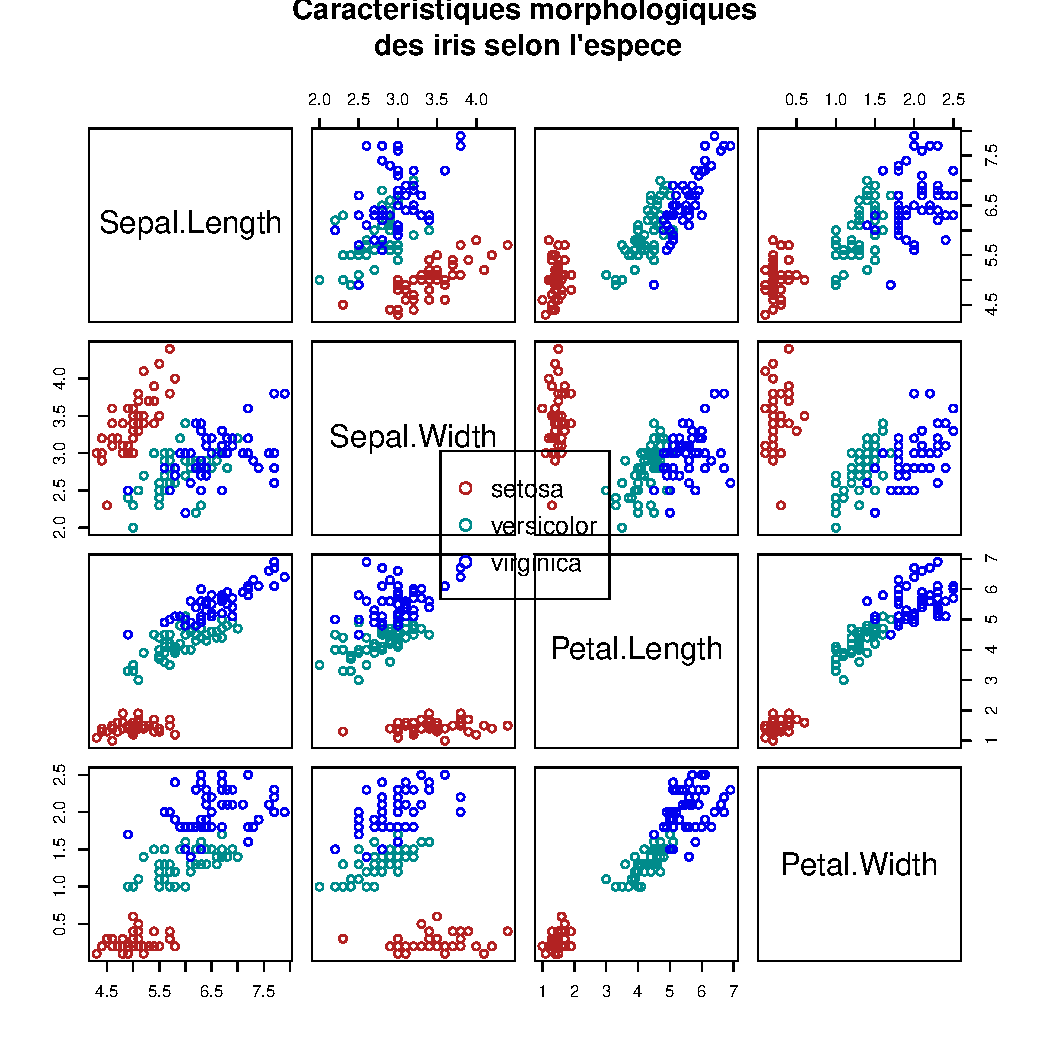
\includegraphics[width=0.35\textwidth]{Iris_selon_espece.pdf}
    \captionof{figure}{Représentation des individus dans les plans formés de $2$ variables quantitatives (Iris)}\label{fig_iris_selon_espece}
\endgroup

Nous avons commencé par représenter les individus dans le premier plan factoriel sans tenir compte de l'espèce (à gauche dans la figure \ref{fig_iris_ex_base_et_individus_u1_u2_sans_avec_dist}). On constate que le premier axe factoriel traduit principalement les variables \texttt{petal length} et \texttt{petal width} tandis que le deuxième axe factoriel semble traduire la variable \texttt{sepal width}. Par ailleurs, le jeu de données semble principalement comporter $2$ groupes de points.

\begingroup
   \centering
   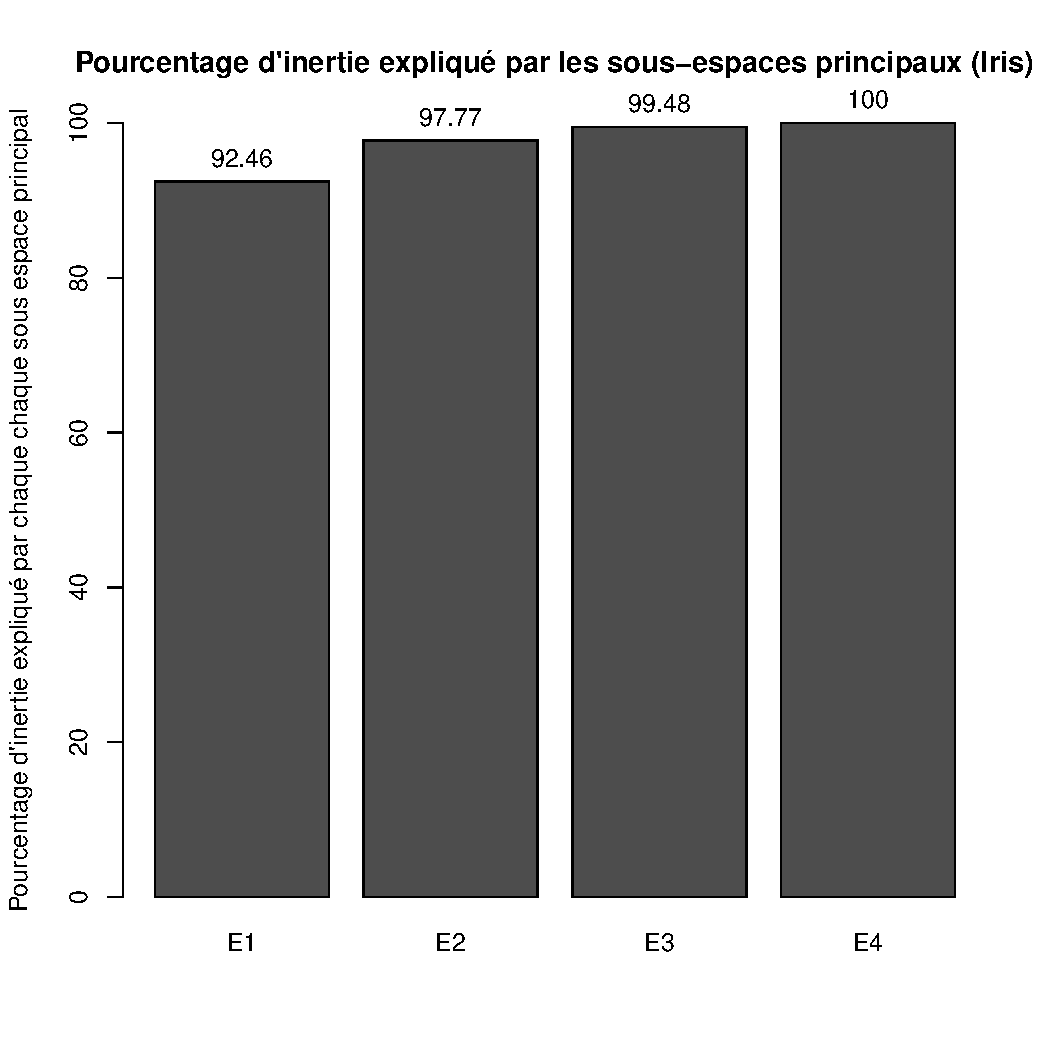
\includegraphics[width=0.35\textwidth]{Iris_batons_valeurs_propres_cumul.pdf}
    \captionof{figure}{Pourcentage d'inertie expliquée par les sous-espaces principaux (Iris)}\label{fig_Iris_batons_valeurs_propres_cumul}
\endgroup

Afin de savoir si ces deux groupes de données sont liés aux espèces des individus, nous avons également représenté ces derniers en tenant compte de ce paramètre (à droite dans la figure \ref{fig_iris_ex_base_et_individus_u1_u2_sans_avec_dist}). Ainsi, il s'avère que l'un des deux groupes est constitué des individus de l'espèce \texttt{setosa}. Les membres de l'autre groupe ont pour espèce, soit \texttt{versicolor}, soit \texttt{virginica}.

Si l'on recherche une partition de données avec $2$ classes, on peut s'attendre à voir que les individus d'une classe ont pour espèce \texttt{setosa} tandis que les individus de l'autre classe sont, soit d'espèce \texttt{versicolor}, soit d'espèce \texttt{virginica}.

\begingroup
	\centering
   \begin{minipage}[c]{0.23\textwidth}
      \centering 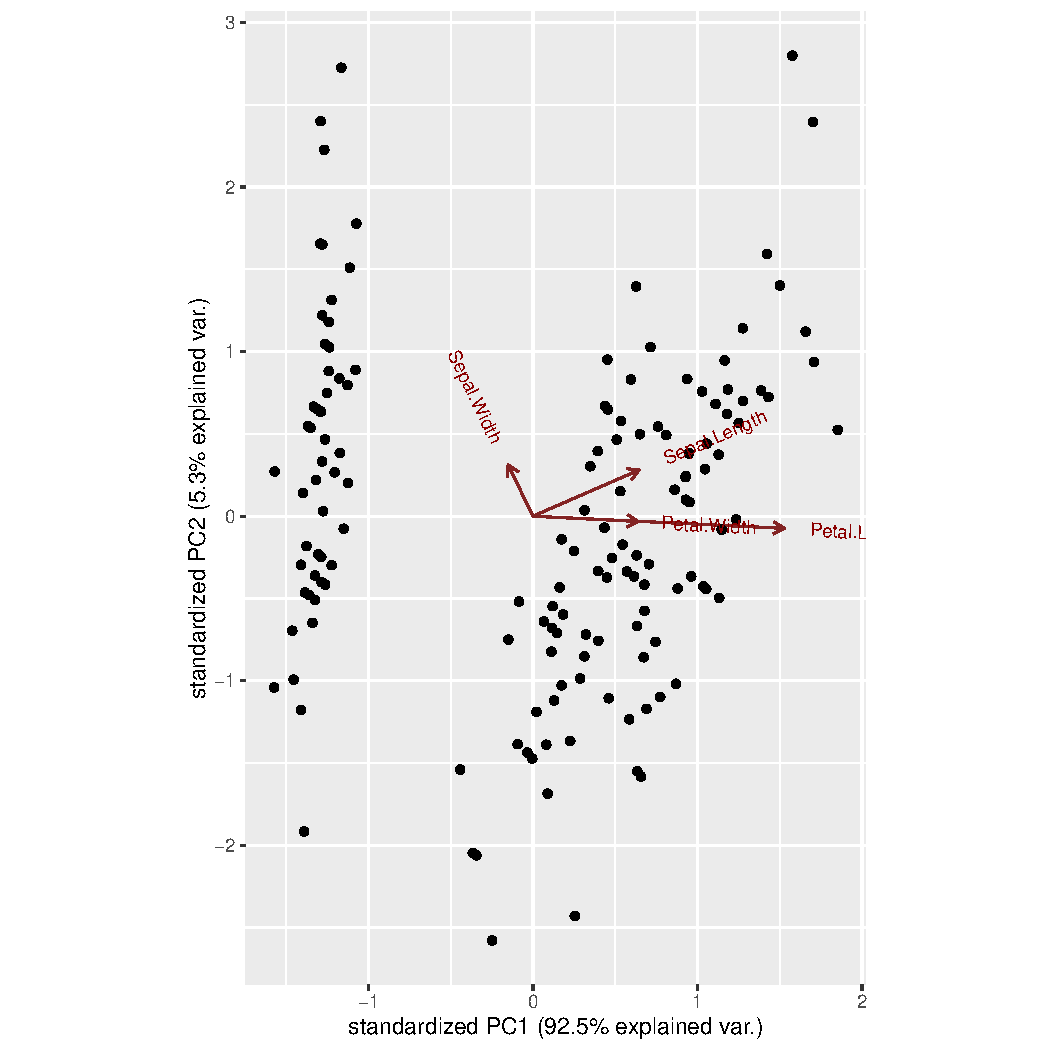
\includegraphics[width=\textwidth]{Iris_ex_base_et_individus_u1_u2_sans_dist.pdf}
   \end{minipage}\hfill
   \begin{minipage}[c]{0.23\textwidth}   
      \centering 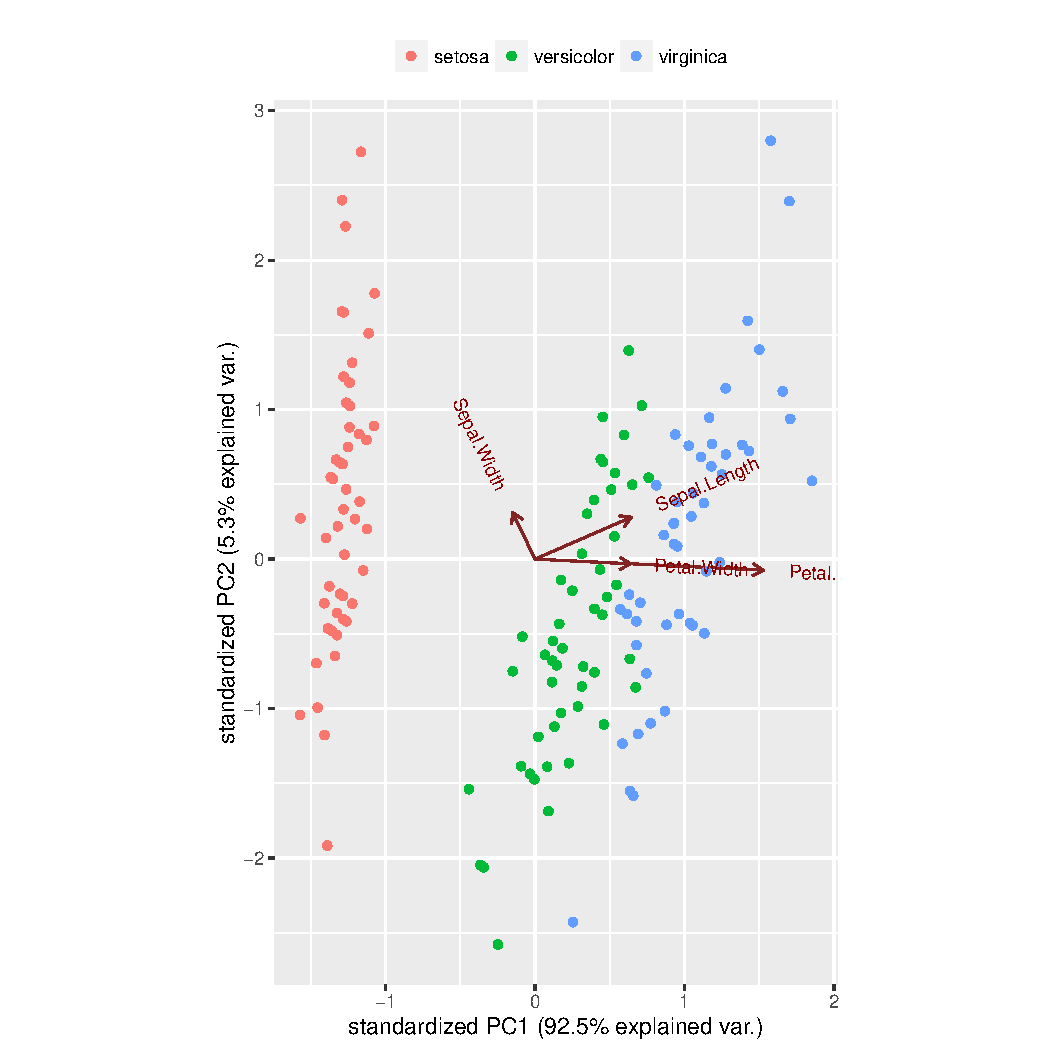
\includegraphics[width=\textwidth]{Iris_ex_base_et_individus_u1_u2_avec_dist.pdf}
   \end{minipage}
    \captionof{figure}{Représentation des individus dans le premier plan factoriel sans tenir compte (à gauche) / en tenant compte (à droite) de l'espèce (Iris)} \label{fig_iris_ex_base_et_individus_u1_u2_sans_avec_dist}
\endgroup


\subsection{Données Crabs}
\label{subsec_visualisation_donnes_crabs}
Le jeu de données \texttt{Crabs} contient des mesures de $4$ variables quantitatives \texttt{FL2}, \texttt{RW2}, \texttt{CL2} et \texttt{BD2} de $200$ crabes : $50$ mâles bleu \texttt{M/B}, $50$ mâles orange $50$ \texttt{M/O}, $50$ femelles bleu \texttt{F/B} et $50$ femelles orange \texttt{F/O}.

Tout d'abord, nous avons commencé par représenter les individus de l'échantillon selon leurs couleurs et leurs sexes, tour à tour, en fonction de $2$ variables quantitatives parmi les $4$ à notre disposition (figure \ref{fig_crabs_selon_sexe_et_espece}). Il semble que les individus de différentes couleurs ou de différents sexes sont distinguables via les $4$ variables quantitatives.

Ensuite, nous avons effectué une \texttt{ACP} sur les $4$ variables quantitatives. Les pourcentages d'inertie expliquée par les sous-espaces principaux sont consultables dans la figure \ref{fig_crabs_batons_valeurs_propre_cumul}. Nous constatons que l'inertie expliquée par le sous espace vectoriel $E_1$ (le premier plan factoriel) est de $92.35 \geq 80$. Ainsi, cela nous a incités à représenter les données dans le premier plan factoriel.

Nous avons commencé par représenter les individus dans le premier plan factoriel sans tenir compte de la couleur et du sexe (à gauche dans la figure \ref{fig_crabs_ex_base_et_individus_u1_u2_sans_avec_dist}). On observe que le premier axe factoriel traduit principalement les variables \texttt{FL2}, \texttt{BD2} et \texttt{CL2} tandis que le deuxième axe factoriel semble traduire la variable \texttt{RW2}. Graphiquement, le jeu de données semble principalement comporter $2$ groupes de points.

\begingroup
   \centering
   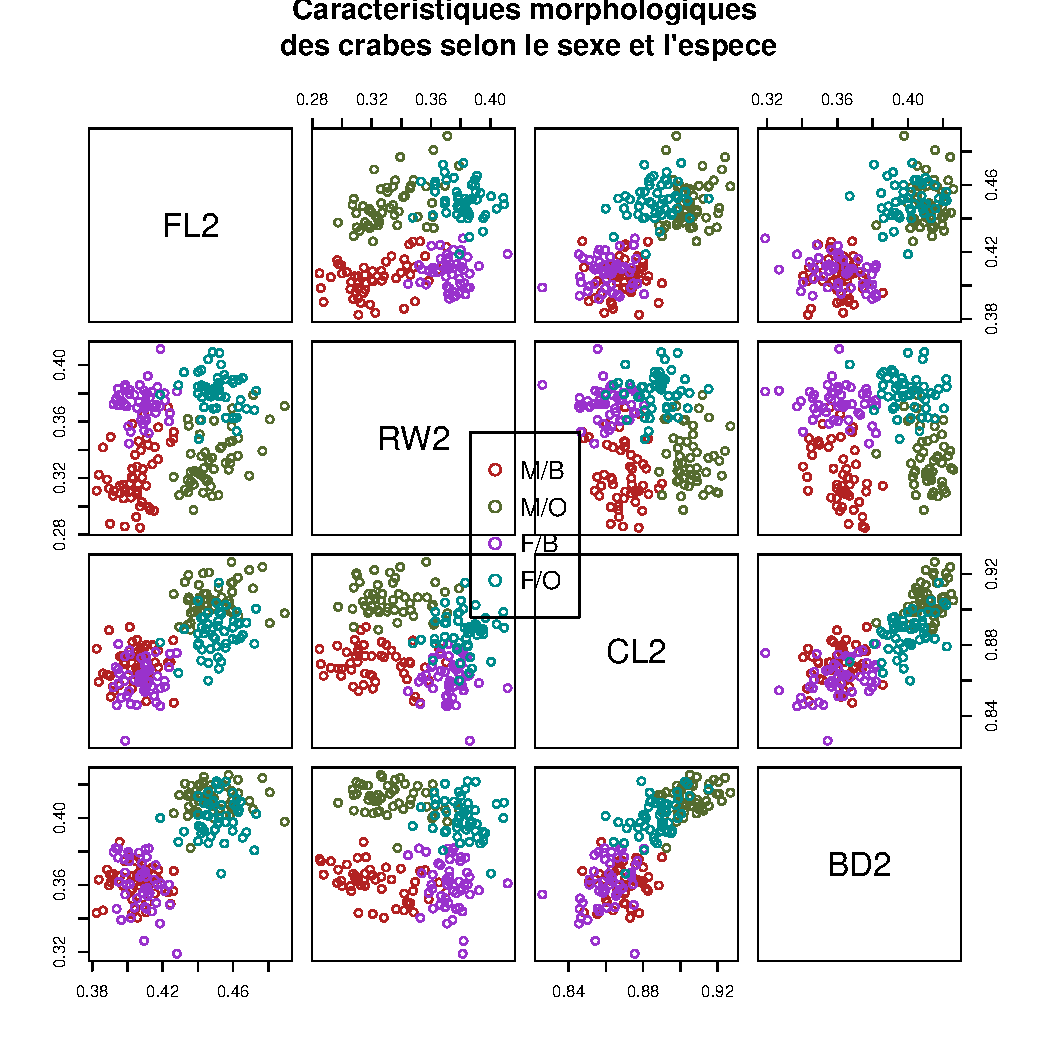
\includegraphics[width=0.35\textwidth]{Crabs_selon_sexe_et_espece.pdf}
    \captionof{figure}{Représentation des individus dans les plans formés de $2$ variables quantitatives (Crabs)}\label{fig_crabs_selon_sexe_et_espece}
\endgroup

Afin de savoir si ces deux groupes de points sont liés aux couleurs ou aux sexes des individus, nous avons également représenté ces derniers en tenant compte de ces paramètres (à droite dans la figure \ref{fig_crabs_ex_base_et_individus_u1_u2_sans_avec_dist}). Il s'avère que l'un des deux groupes est constitué des individus \texttt{F/O} et \texttt{M/O}. Les membres de l'autre groupe sont, soit des \texttt{F/B}, soit des \texttt{M/B}. Ainsi, un groupe contient des individus \texttt{O} tandis que l'autre contient des individus \texttt{B}.

\begingroup
   \centering
   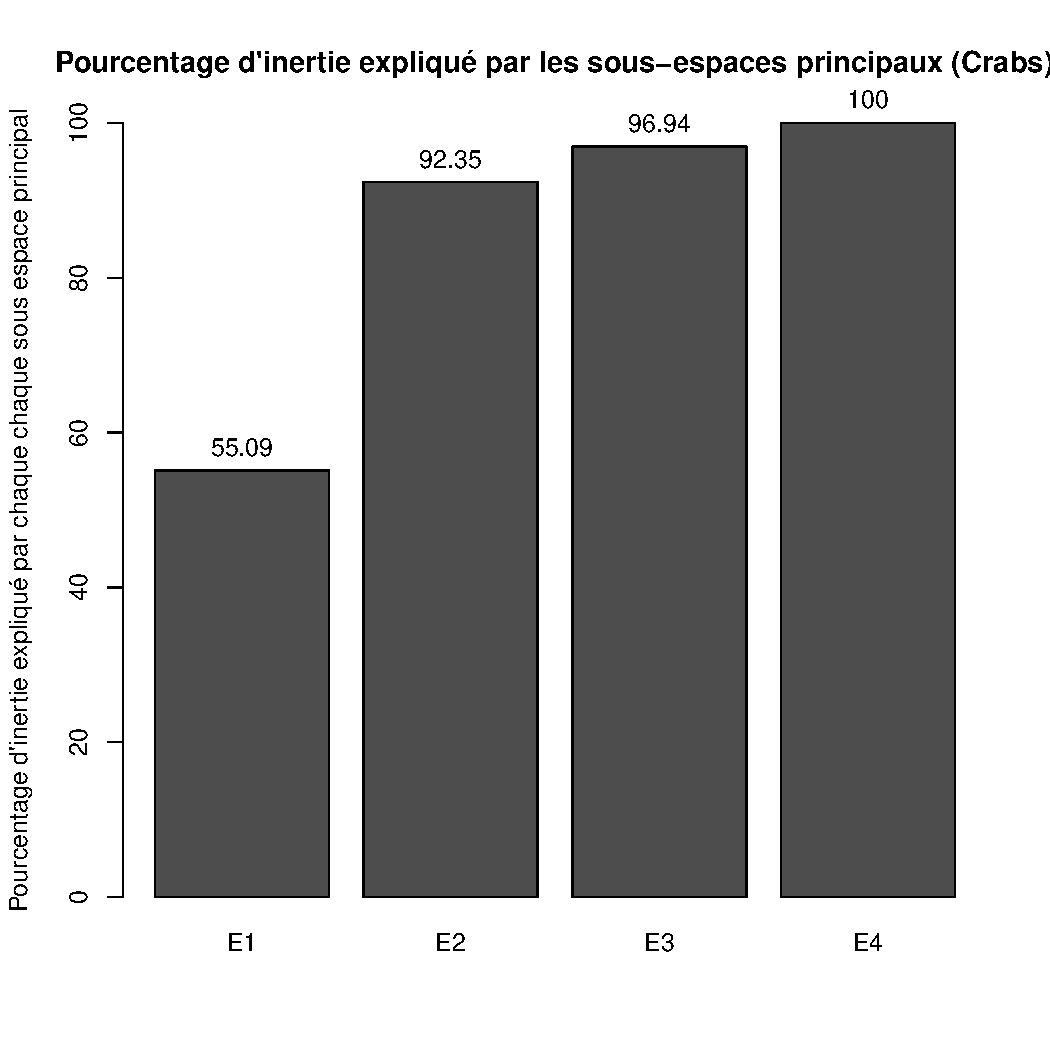
\includegraphics[width=0.35\textwidth]{Crabs_batons_valeurs_propre_cumul.pdf}
    \captionof{figure}{Pourcentage d'inertie expliquée par les sous-espaces principaux (Crabs)}\label{fig_crabs_batons_valeurs_propre_cumul}
\endgroup

Si l'on recherche une partition de données avec $2$ classes, on peut s'attendre à voir que les individus d'une classe sont principalement des \texttt{O} tandis que les individus de l'autre classe sont majoritairement des \texttt{B}.

\begingroup
	\centering
   \begin{minipage}[c]{0.23\textwidth}
      \centering 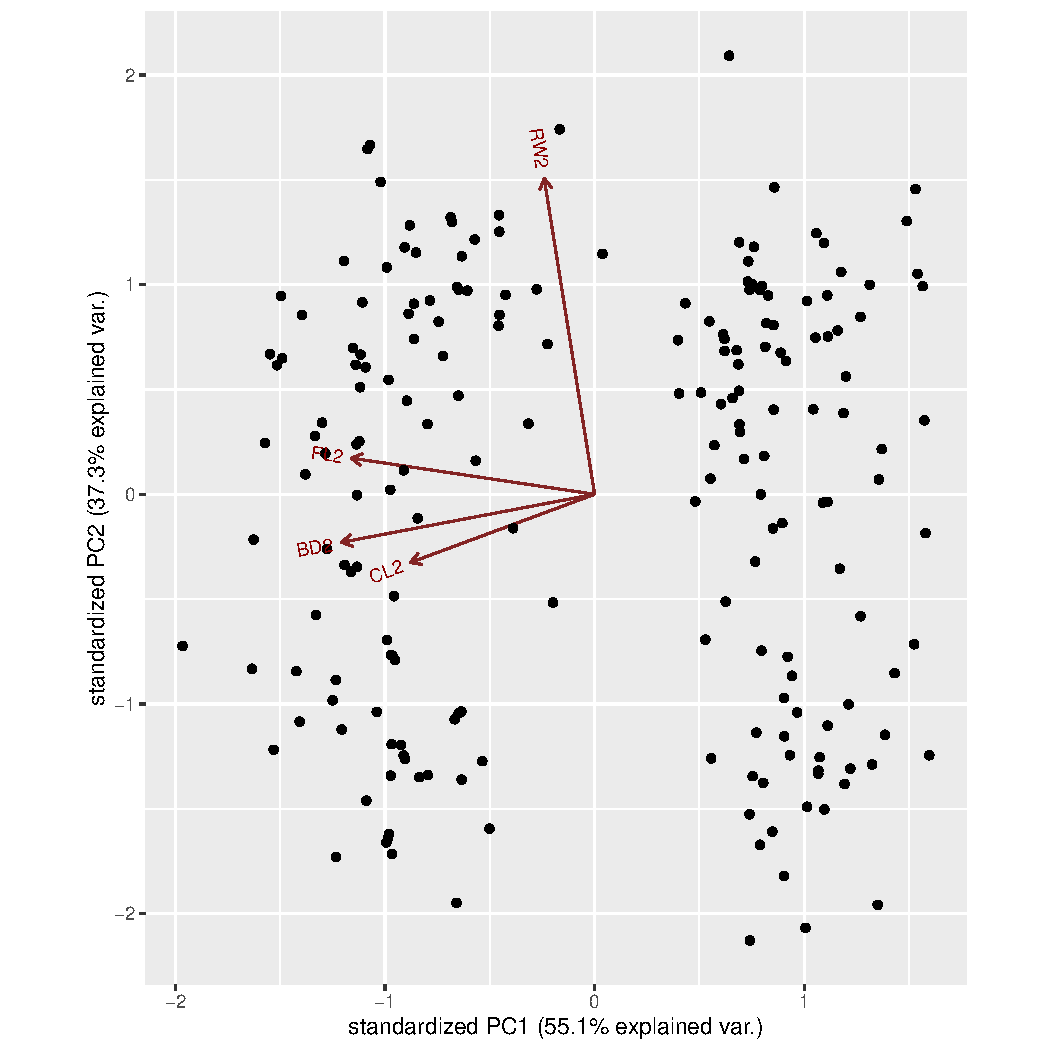
\includegraphics[width=\textwidth]{Crabs_ex_base_et_individus_u1_u2_sans_dist.pdf}
   \end{minipage}\hfill
   \begin{minipage}[c]{0.23\textwidth}   
      \centering 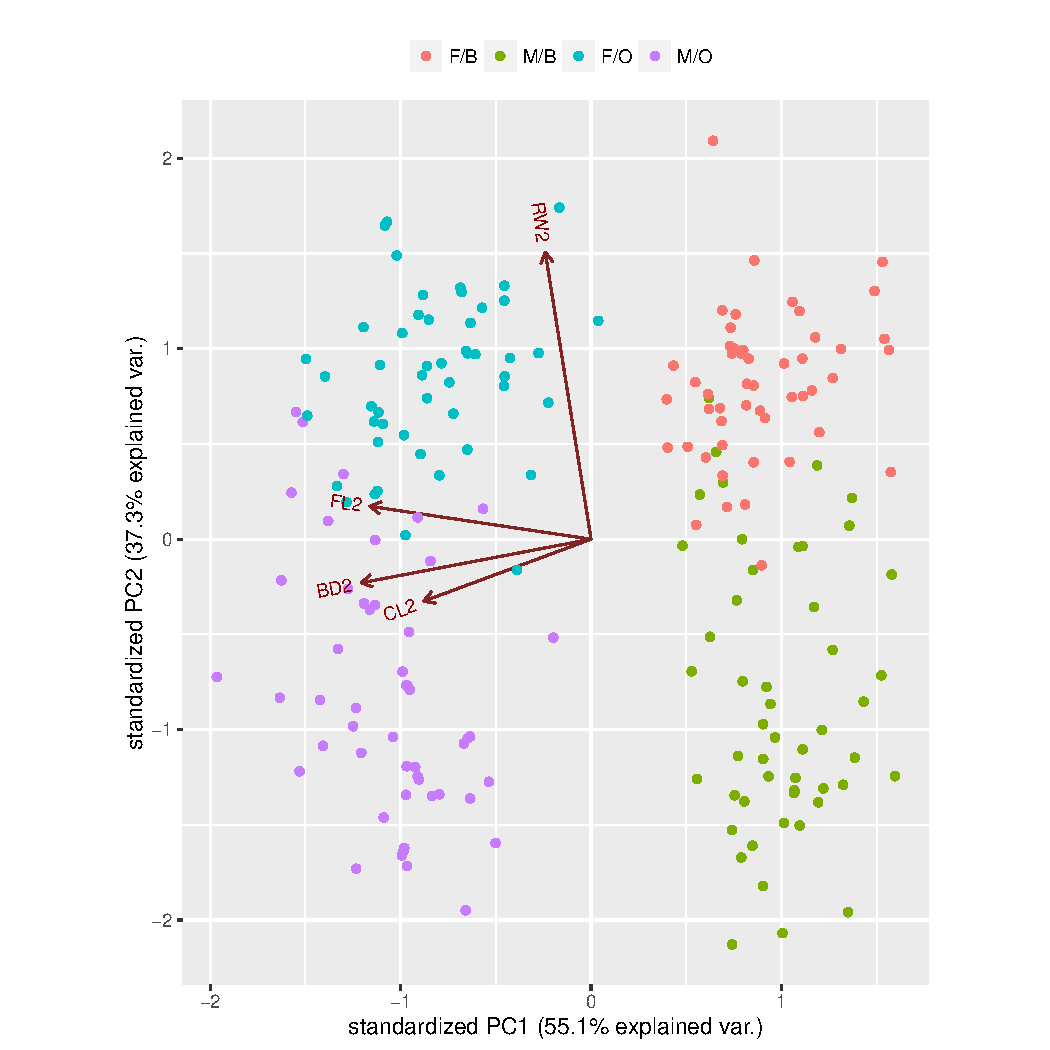
\includegraphics[width=\textwidth]{Crabs_ex_base_et_individus_u1_u2_avec_dist.pdf}
   \end{minipage}
    \captionof{figure}{Représentation des individus dans le premier plan factoriel sans tenir (à gauche) / en tenant (à droite) compte de l'espèce et du sexe (Crabs)} \label{fig_crabs_ex_base_et_individus_u1_u2_sans_avec_dist}
\endgroup


\subsection{Données Mutations}
\label{subsec_visualisation_donnes_mutations}
Le jeu de données \texttt{Mutations} est un tableau de dissimilarités $\Delta$ sur $n = 20$ espèces. Les dissimilarités entre deux individus de l'échantillon ont été calculées en se basant sur les différentes positions des acides aminés de la protéine \texttt{Cytochrome C}.

Pour commencer, nous avons calculé une représentation euclidienne des données en $d = 2$ variables par Analyse Factorielle d'un Tableau de Dissimilarités (\texttt{AFTD}). Les résultats obtenus sont consultables dans la figure \ref{fig_mutations_test_1}. 

Dans ce graphique (figure \ref{fig_mutations_test_1}), on peut remarquer que l'homme est proche du singe. De même, le pigeon est proche du canard. De plus, le cheval est proche du chien. Ces résultats semblent plutôt cohérents.

\begingroup
   \centering
   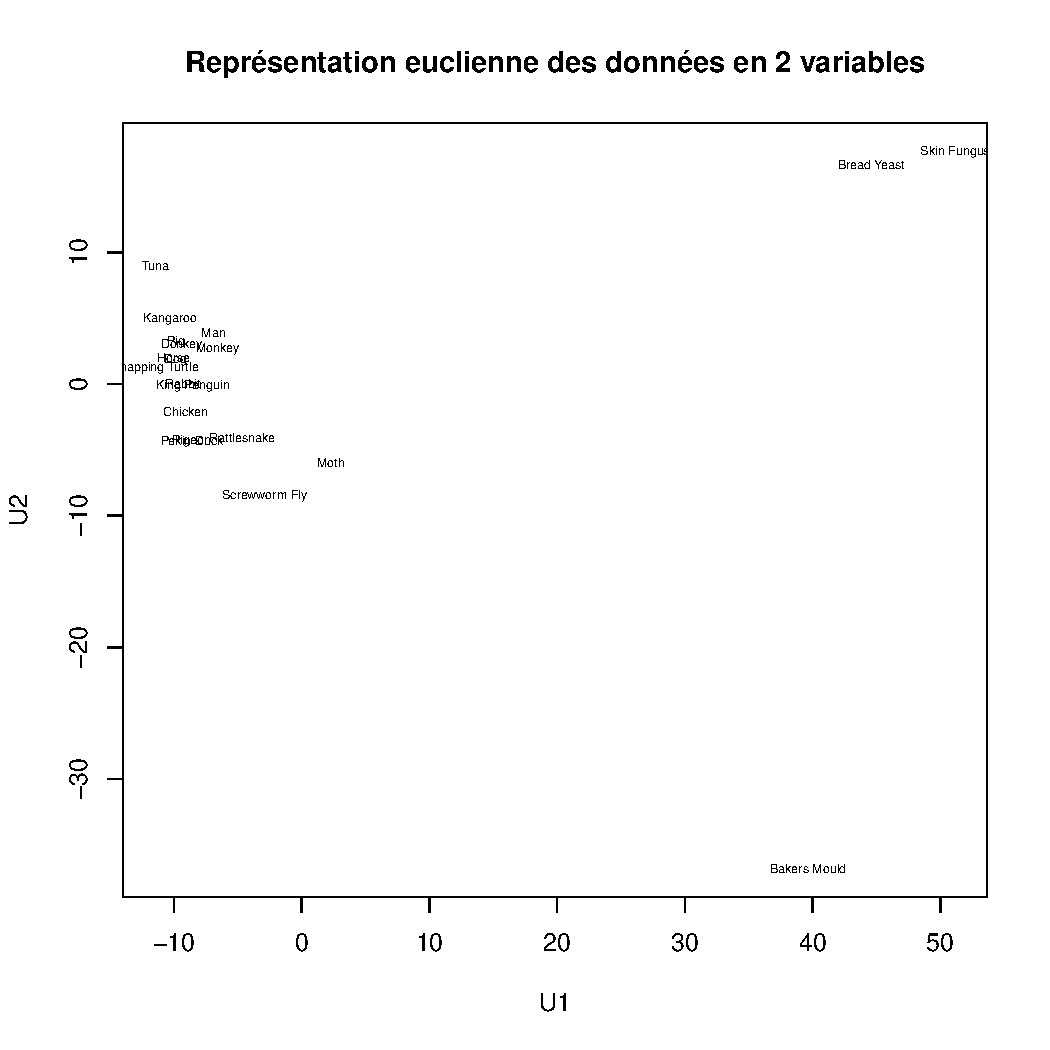
\includegraphics[width=0.35\textwidth]{mutations_test_1.pdf}
    \captionof{figure}{Représentation euclidienne des données en $d=2$ par AFTD sans ajout de constante préalable}\label{fig_mutations_test_1}
\endgroup

Toutefois, on constate que les valeurs propres ordonnées de la matrice $\frac{1}{n}W = -\frac{1}{2n}Q_n \Delta^2 Q_n$, où $Q_n = I_n - \frac{1}{n} U_n$, ne sont pas toutes positives ou nulles. Effectivement, la dernière valeur propre $\lambda_{20} = -72.75$ représente en valeur absolue plus de $\frac{1}{10}$ de la cinquième valeur propre ($\lambda_{5} = 675.04$). Nous jugeons que cela n'est pas négligeable et peut, par conséquent, avoir un impact sur la qualité de la représentation. Par conséquent, nous avons décidé de ne plus appliquer directement l'\texttt{AFTD} sur le jeu de données \texttt{Mutations}.  

Ainsi, nous avons choisi d'ajouter une constante que l'on nommera $c^\ast$ à la dissimilarité initiale $\Delta$ en vue de la transformer en une distance, avant d'appliquer l'\texttt{AFTD}. 

Les pourcentages d'inertie expliquée par les sous-espaces principaux sont consultables dans la figure \ref{fig_mutations_test_2_pourc_iner_cumul}. Nous constatons que l'inertie expliquée par le sous espace vectoriel $E_1$ (le premier plan factoriel) est de $91.1 \geq 80$. Ainsi, la représentation euclidienne des données dans un espace de dimension de $d = 2$ semble raisonnable. 

\begingroup
   \centering
   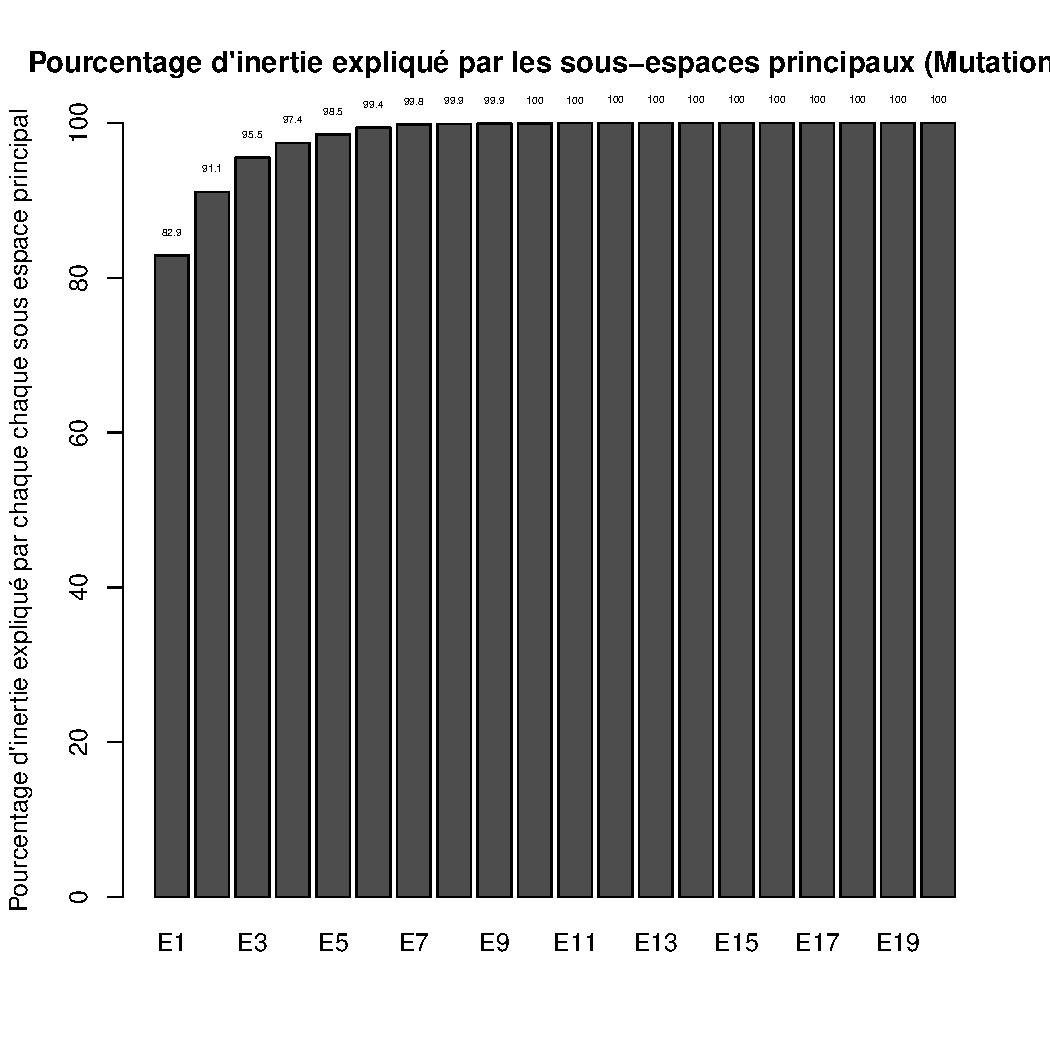
\includegraphics[width=0.35\textwidth]{mutations_test_2_pourc_iner_cumul.pdf}
    \captionof{figure}{Pourcentage d'inertie expliquée par les sous-espaces principaux (Mutations)}\label{fig_mutations_test_2_pourc_iner_cumul}
\endgroup

Les résultats obtenus sont consultables dans la figure \ref{fig_mutations_test_2}. A l'instar de la figure \ref{fig_mutations_test_1}, le graphique semble cohérent. Effectivement, il est très semblable à celui obtenu dans la figure \ref{fig_mutations_test_1}.

\begingroup
   \centering
   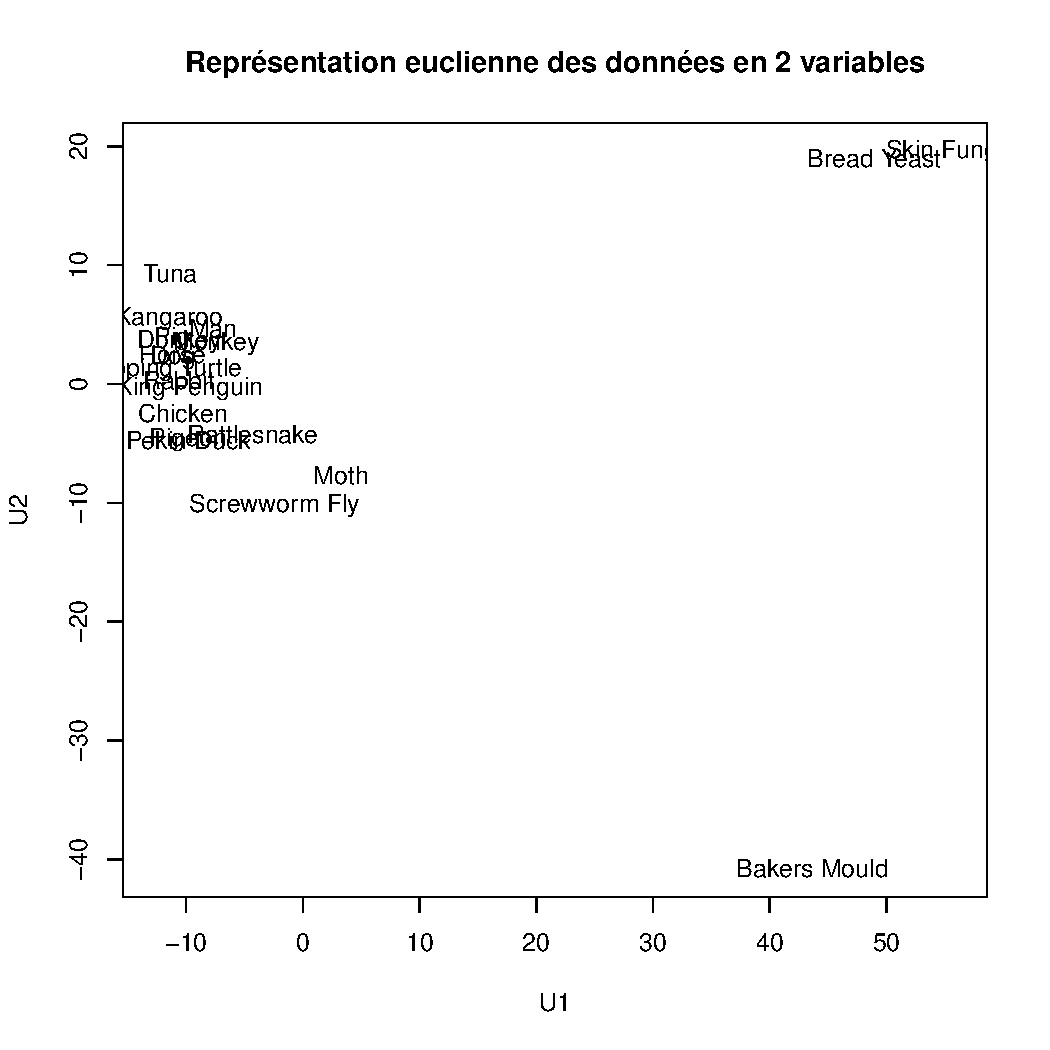
\includegraphics[width=0.35\textwidth]{mutations_test_2.pdf}
    \captionof{figure}{Représentation euclidienne des données en $d=2$ par AFTD avec ajout de constante préalable}\label{fig_mutations_test_2}
\endgroup

Par ailleurs, afin de prendre conscience de la qualité de la représentation, nous avons tracé le diagramme de \texttt{Shepard} à partir de la représentation euclidienne des données dans un espace à $d = 2$ dimensions obtenue via l'\texttt{AFTD}. L'utilisation de ce diagramme est cohérente puisque l'\texttt{AFTD} vise à minimiser le critère $\sum_{i \in \Omega} \sum_{i' \in \Omega}(\delta_{ii'}^{2} - d_{ii'}^{2})$, où $d_{ii'}$ représente la distance entre les individus $i$ et $i'$ calculée à partir de la représentation euclidienne $X$ obtenue via l'\texttt{AFTD} et où $\delta_{ii'}$ représente la dissimilarité initiale entre les individus $i$ et $i'$. Le diagramme de \texttt{Shepard} permet de représenter la dissimilarité au sein de chaque couple de deux individus en fonction de leur distance. Ainsi, plus la représentation est bonne, plus le nuage de points est proche de la bissectrice.

Le diagramme de \texttt{Shepard} obtenu est consultable à gauche dans la figure \ref{fig_mutations_test_2_4_shepard}. Il est évidemment difficile d'interpréter directement ce graphique. Afin de pouvoir le faire de manière pertinente, nous avons décidé de réaliser un diagramme de \texttt{Shepard} (à droite dans la figure \ref{fig_mutations_test_2_4_shepard}) à partir d'une représentation euclidienne dans un espace de $d = 5$ dimensions obtenue via l'\texttt{AFTD} avec ajout d'une constante $c^{\ast}$ au préalable.

\begingroup
	\centering
   \begin{minipage}[c]{0.23\textwidth}
      \centering 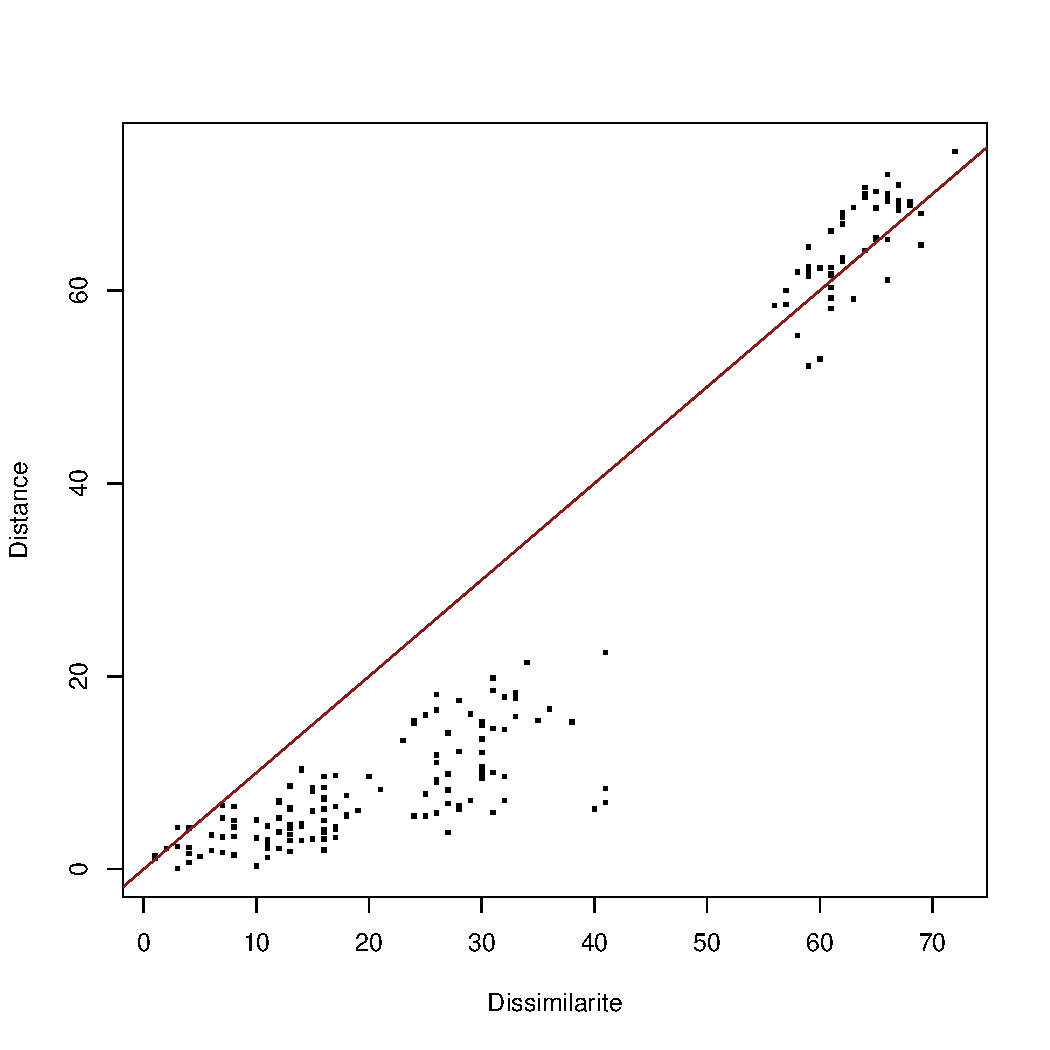
\includegraphics[width=\textwidth]{mutations_test_2_shepard.pdf}
   \end{minipage}\hfill
   \begin{minipage}[c]{0.23\textwidth}   
      \centering 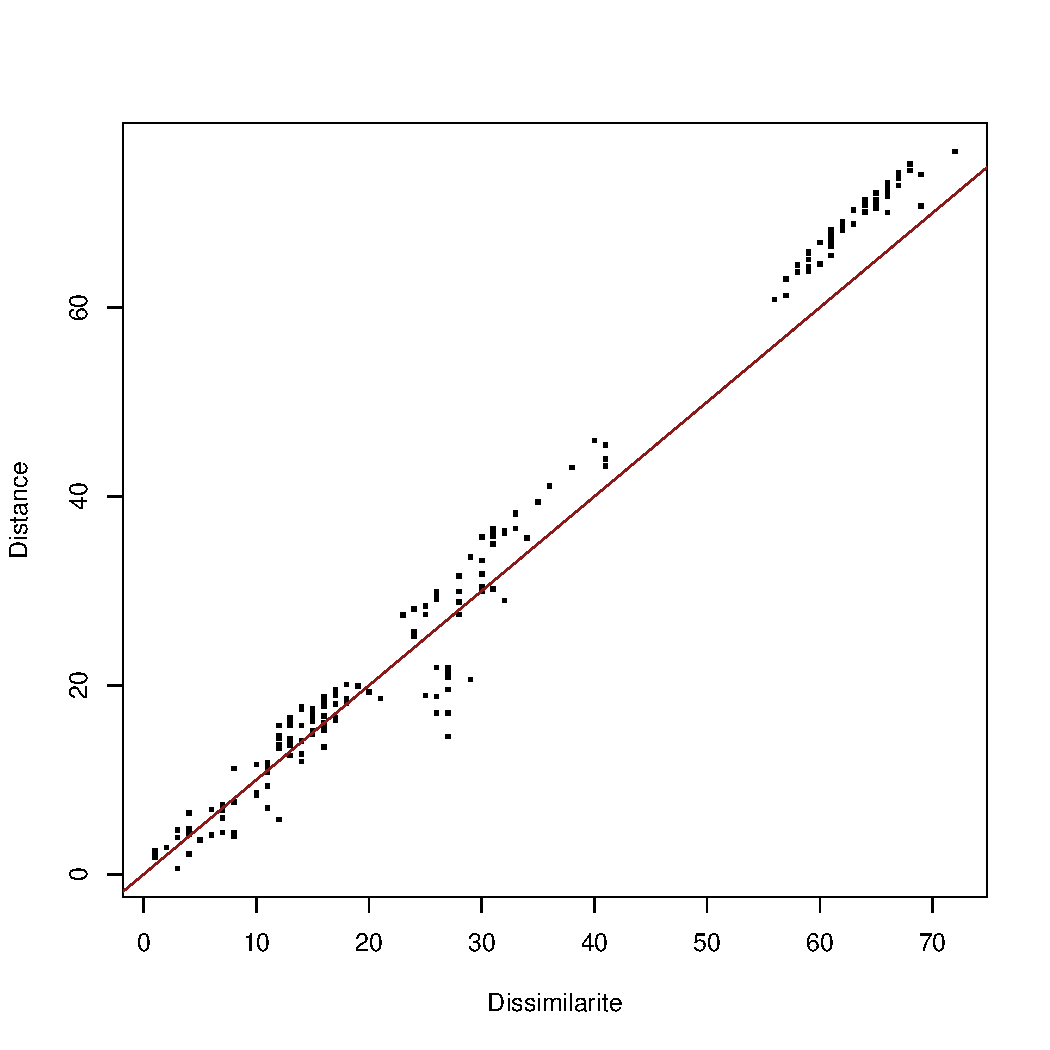
\includegraphics[width=\textwidth]{mutations_test_4_shepard.pdf}
   \end{minipage}
    \captionof{figure}{Diagramme de Shepard associé à la représentation euclidienne des données en d=2 (à gauche) / en d=5 (à droite) (Crabs)} \label{fig_mutations_test_2_4_shepard}
\endgroup


Évidemment, nous constatons que le nuage de points à gauche dans la figure \ref{fig_mutations_test_2_4_shepard} est plus proche de la bissectrice que celui à droite dans la figure \ref{fig_mutations_test_2_4_shepard} : cela est logique puisque on a perdu moins d'informations à droite dans la figure \ref{fig_mutations_test_2_4_shepard} qu'à gauche dans la figure \ref{fig_mutations_test_2_4_shepard}. Toutefois, la représentation dans un espace à dimensions $5$ est difficilement graphiquement exploitable. Par ailleurs, on peut également ajouter que la baisse de la qualité de la représentation est "raisonnable" compte tenu du gain apporté par la représentation dans un plan. Ainsi, de ce fait, nous continuerons à utiliser la représentation dans un espace à $d = 2$ dimensions dans ce rapport. 

\section{Classification hiérarchique}
\label{sec_classification_hierarchique}

\subsection{Données Mutations}
\label{subsec_class_hier_mutations}

Dans cette sous-section \ref{subsec_class_hier_mutations}, nous allons étudier le jeu de données \texttt{Mutations} à travers une Classification Ascendante Hiérarchique (CAH). Pour ce faire, nous allons utiliser le tableau de dissimilarités $\Delta$ lui étant associé. 

\begingroup
   \centering
   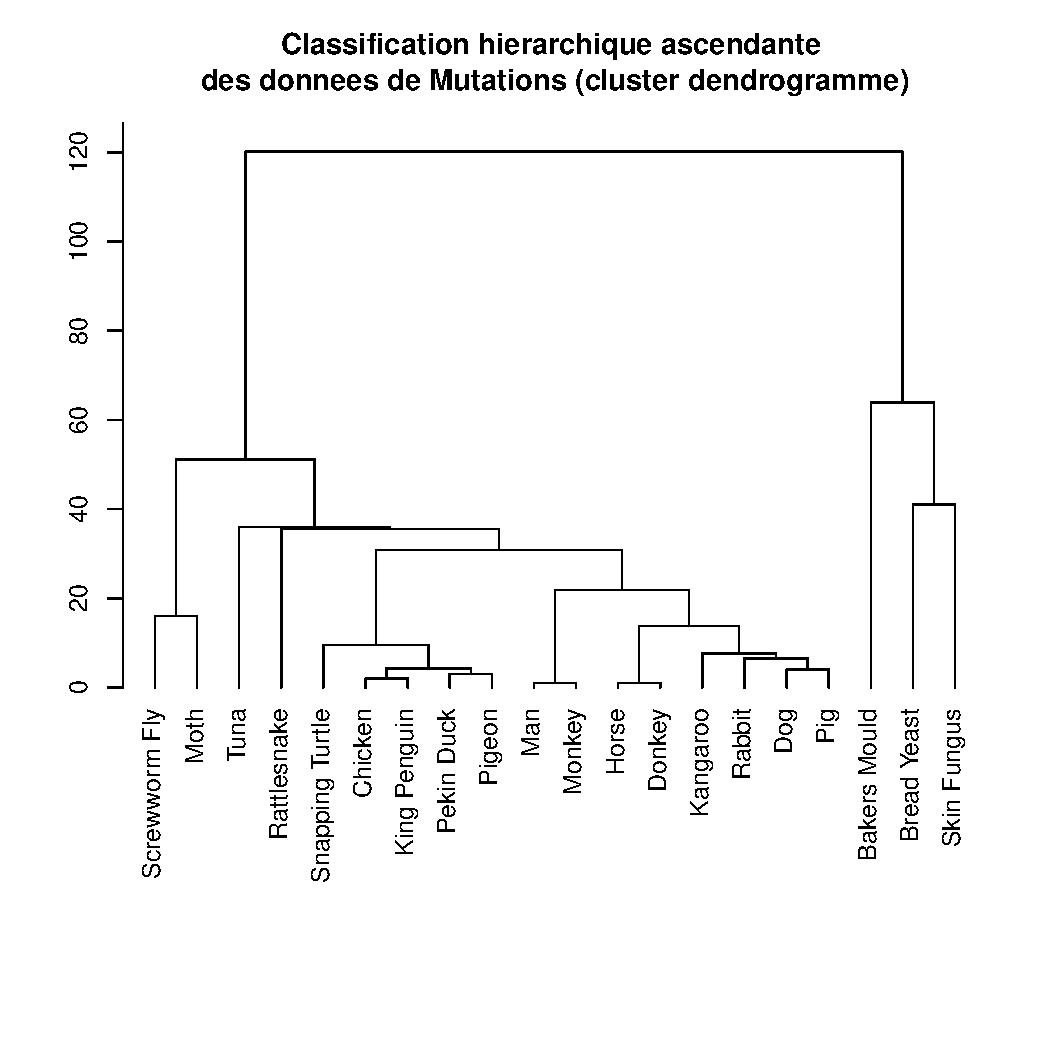
\includegraphics[width=0.35\textwidth]{Mutations_cluster_dendrogramme_ascendante.pdf}
    \captionof{figure}{Dendrogramme de la CAH avec la méthode de Ward (données Mutations)}\label{cha_mut_ward}
\endgroup

La méthode consiste à commencer par considérer une partition constitués de classes qui sont des singletons. A chaque étape, on fusionne des classes suivant un critère d'agrégation jusqu'à l'obtention d'une seule classe constitué de l'ensemble des individus. Les résultats seront représentés graphiquement dans les figures \ref{cha_mut_ward}, \ref{cha_mut_complete}, \ref{cha_mut_mcquitty}, \ref{cha_mut_single}, \ref{cha_mut_median} et \ref{cha_mut_cendroid} via des dendrogrammes symbolisant les hiérarchies indicées obtenues avec les différentes méthodes utilisées.

Suite aux résultats trouvés, on peut observer que les CAH avec les critères d'agrégations de \texttt{McQuitty} (figure \ref{cha_mut_mcquitty}), \texttt{Complete} (figure \ref{cha_mut_complete}) et \texttt{Ward} (figure \ref{cha_mut_ward}) permettent d'obtenir des résultats "très" similaires. Celles avec les critères \texttt{Single} (figure \ref{cha_mut_single}) et \texttt{Median} (figure \ref{cha_mut_median}) donnent des résultats "légèrement" différents (notamment pour les classes \texttt{Bakers Mould} et \texttt{Tuna}). 

\begingroup
   \centering
   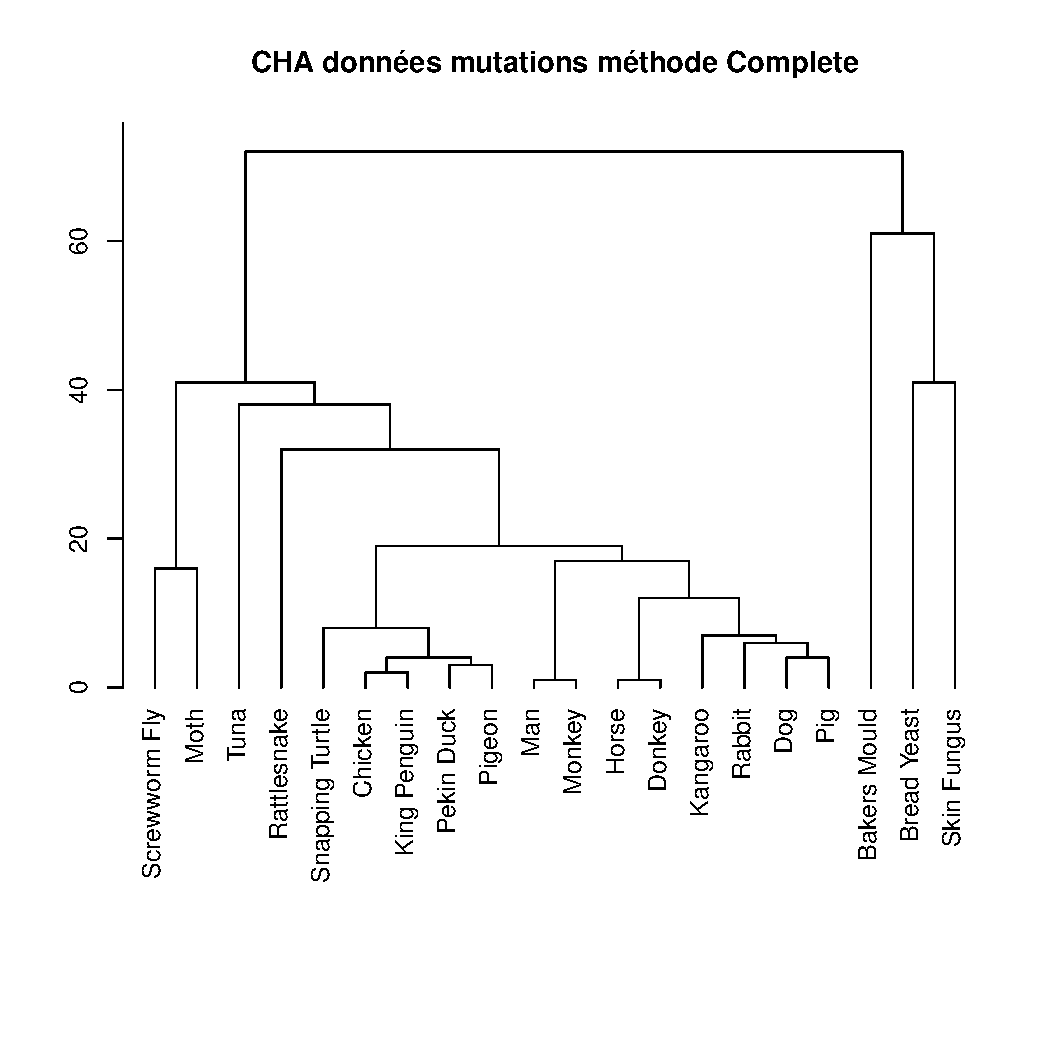
\includegraphics[width=0.35\textwidth]{complete_mut.pdf}
    \captionof{figure}{Dendrogramme avec le critère d'agrégation Complete (Mutations)}\label{cha_mut_complete}
\endgroup

\begingroup
   \centering
   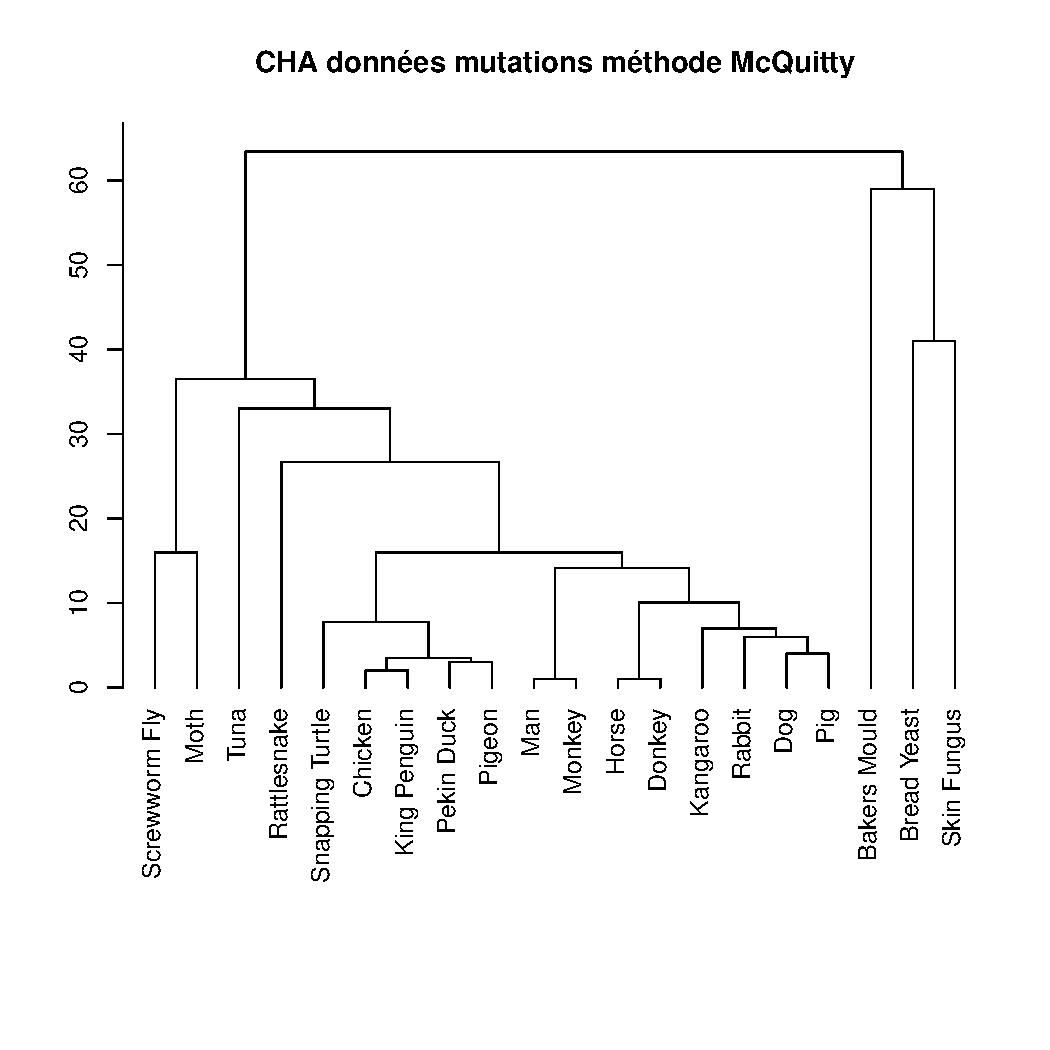
\includegraphics[width=0.35\textwidth]{mcquitty_mut.pdf}
    \captionof{figure}{Dendrogramme avec le critère d'agrégation McQuitty (Mutations)}\label{cha_mut_mcquitty}
\endgroup

\begingroup
   \centering
   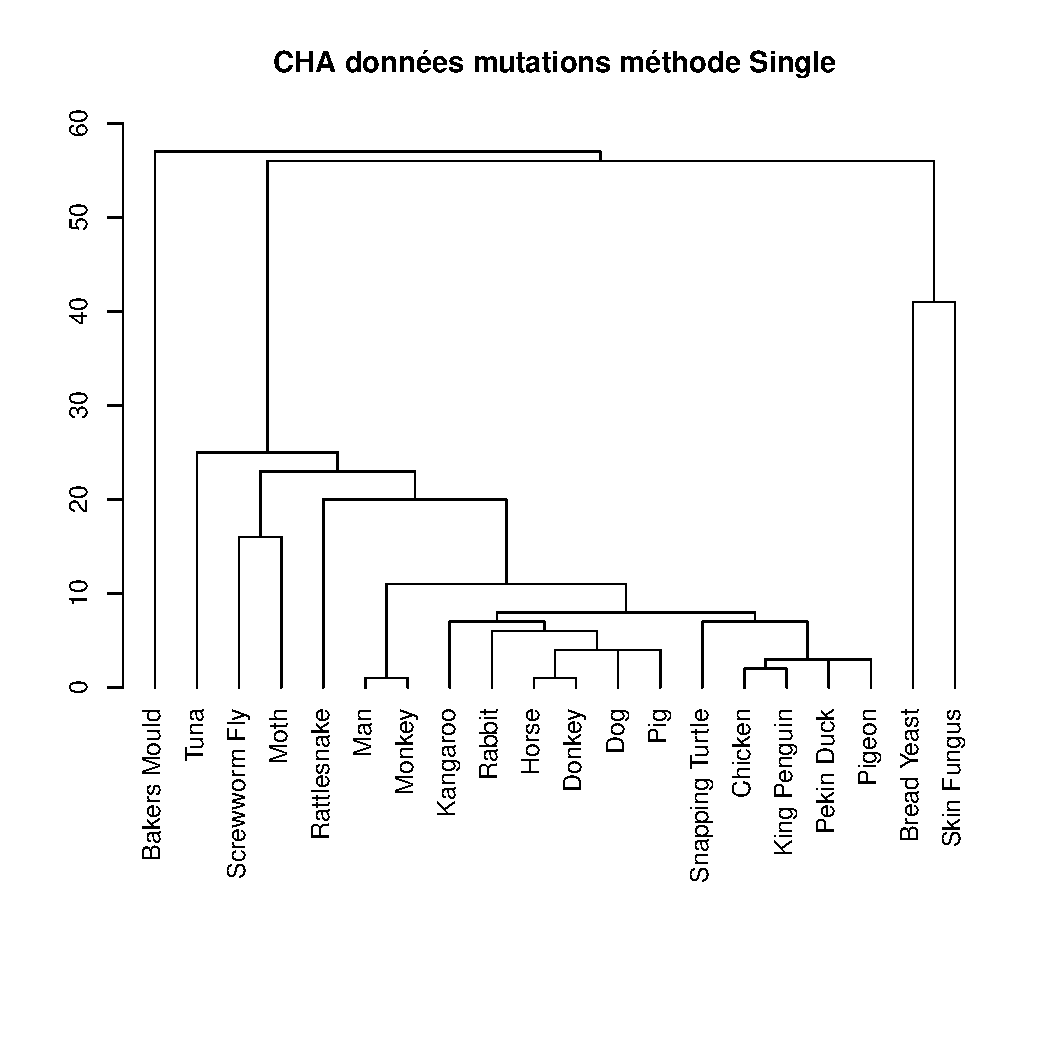
\includegraphics[width=0.35\textwidth]{single_mut.pdf}
    \captionof{figure}{Dendrogramme avec le critère d'agrégation Single (Mutations)}\label{cha_mut_single}
\endgroup

\begingroup
   \centering
   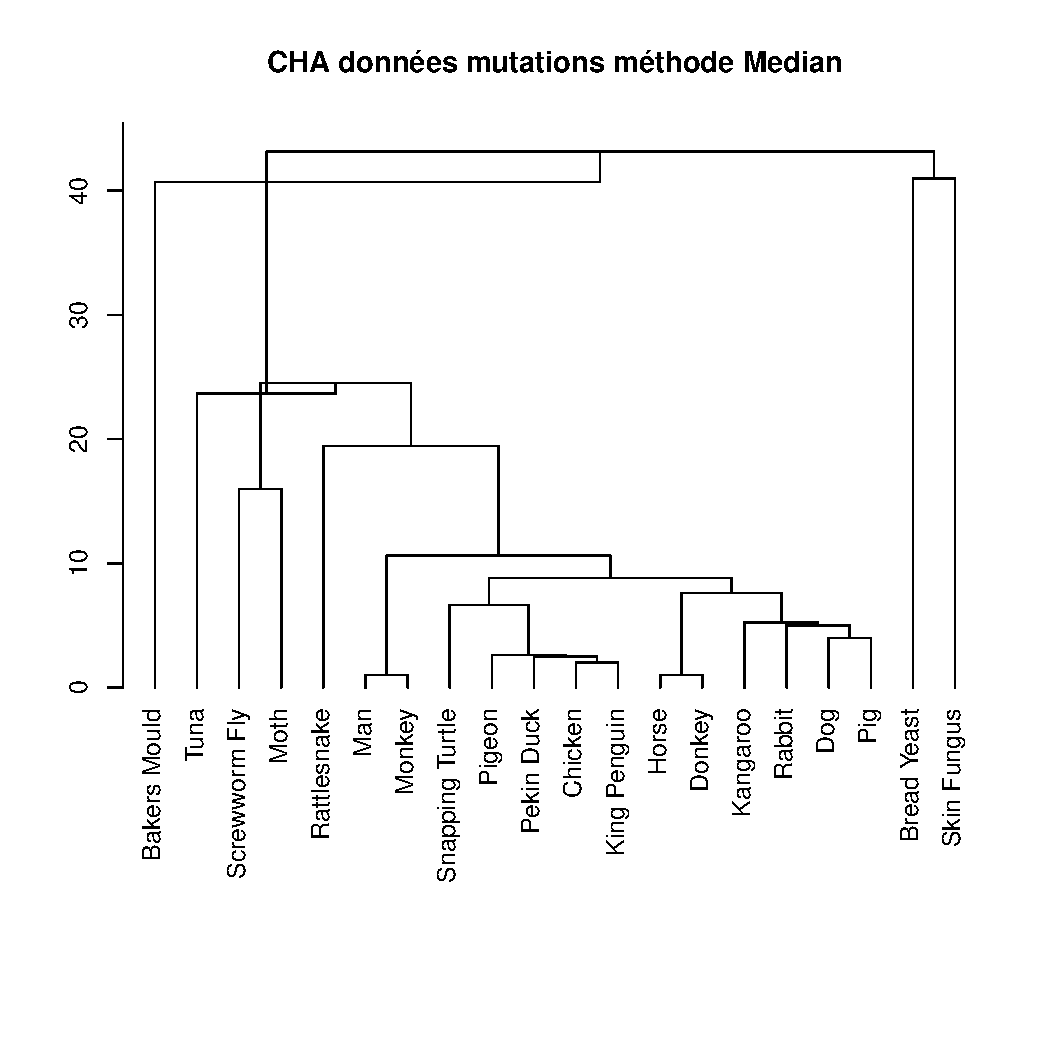
\includegraphics[width=0.35\textwidth]{median_mut.pdf}
    \captionof{figure}{Dendrogramme avec le critère d'agrégation Median (Mutations)}\label{cha_mut_median}
\endgroup

\begingroup
   \centering
   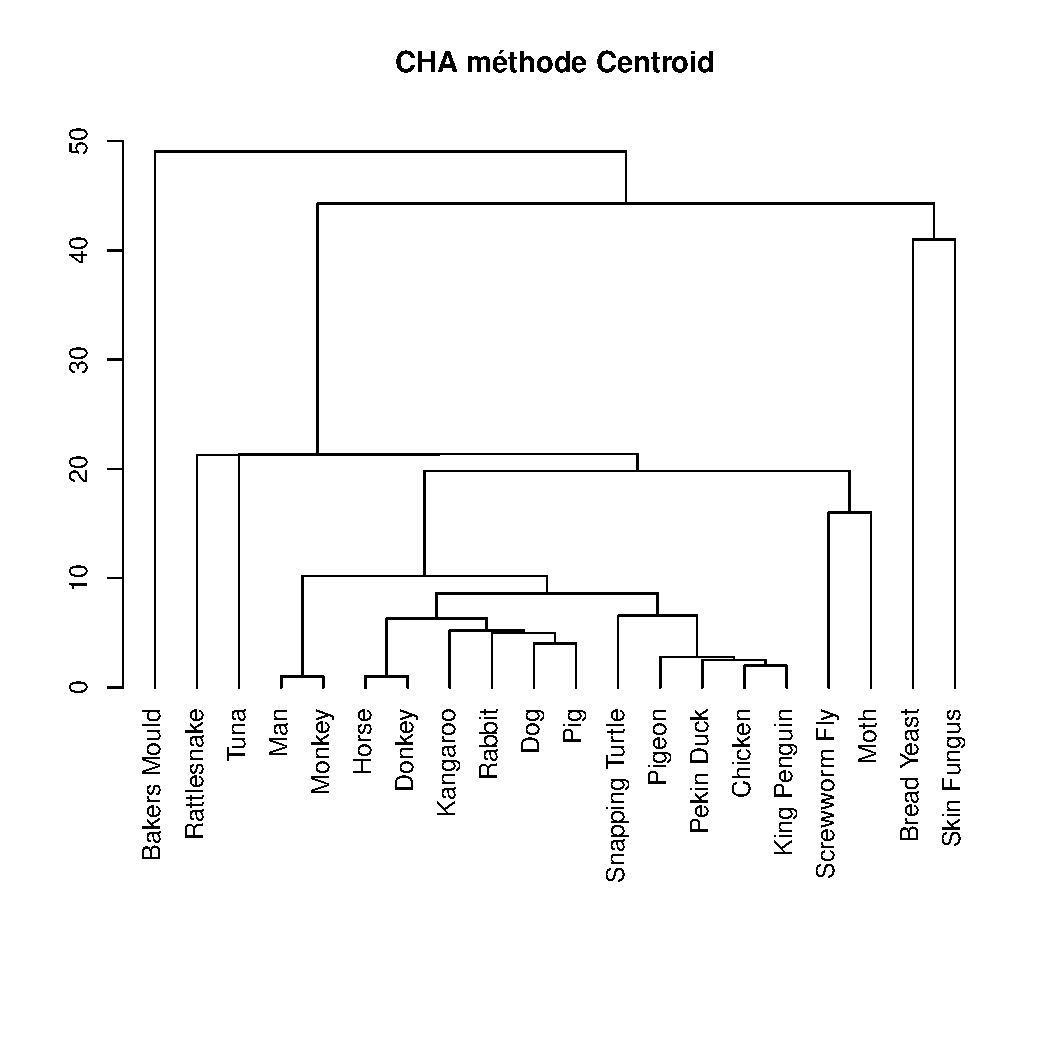
\includegraphics[width=0.35\textwidth]{centroid_mut.pdf}
    \captionof{figure}{Dendrogramme avec le critère d'agrégation Centroid (Mutations)}\label{cha_mut_cendroid}
\endgroup

On notera la présence d'inversions dans le dendrogramme associé au critère \texttt{Median} (figure \ref{cha_mut_median}). Finalement, la méthode \texttt{Centroid} (figure \ref{cha_mut_cendroid}) diffère des autres dendrogrammes sur de "nombreux" points.

En comparant les différents dendrogrammes avec les résultats obtenus précédemment (sous-section \ref{subsec_visualisation_donnes_mutations}), le critère de \texttt{Ward} semble être le plus adapté à nos données. On retrouve d'ailleurs nos $3$ espèces très éloignées des autres : \texttt{Bakers Mould}, \texttt{Bread Yeast} et \texttt{Skin Fungus}.

On pourra noter qu'à chaque étape de la méthode de \texttt{Ward}, on cherche à fusionner deux classes de sorte à augmenter le moins possible le critère d'inertie intra-classe. Ainsi, cette propriété de cette méthode nous incite à continuer de l'utiliser dans la suite de notre étude.

\subsection{Données Iris}

On effectue la CAH sur les données \texttt{Iris} avec le critère d'agrégation de \texttt{Ward} suite aux précédentes remarques.

A l'instar de la sous-section \ref{subsec_visualisation_donnes_iris}, sur le dendrogramme obtenu (figure \ref{cha_iris_ward}), $3$ grandes classes correspondant aux $3$ espèces du jeu de données \texttt{Iris} se distinguent : \texttt{Setosa}, \texttt{Versicolor} et \texttt{Virginica}.

Contrairement à la représentation dans le premier plan factoriel (figure \ref{fig_iris_ex_base_et_individus_u1_u2_sans_avec_dist} dans la sous-section \ref{subsec_visualisation_donnes_iris}), les espèces \texttt{Versicolor} et \texttt{Virginica} sont "facilement" distinguables. De plus, on peut observer que les individus des deux espèces (dans les rectangles vert et bleu de la figure \ref{cha_iris_ward}) sont issus d'un même sous-arbre (branche droite de la racine) : cela semble confirmer le fait que les individus des deux classes précédemment citées sont plus "proches" les uns des autres qu'avec ceux de la troisième classe au sens du critère d'inertie intra-classe. 

\begingroup
   \centering
   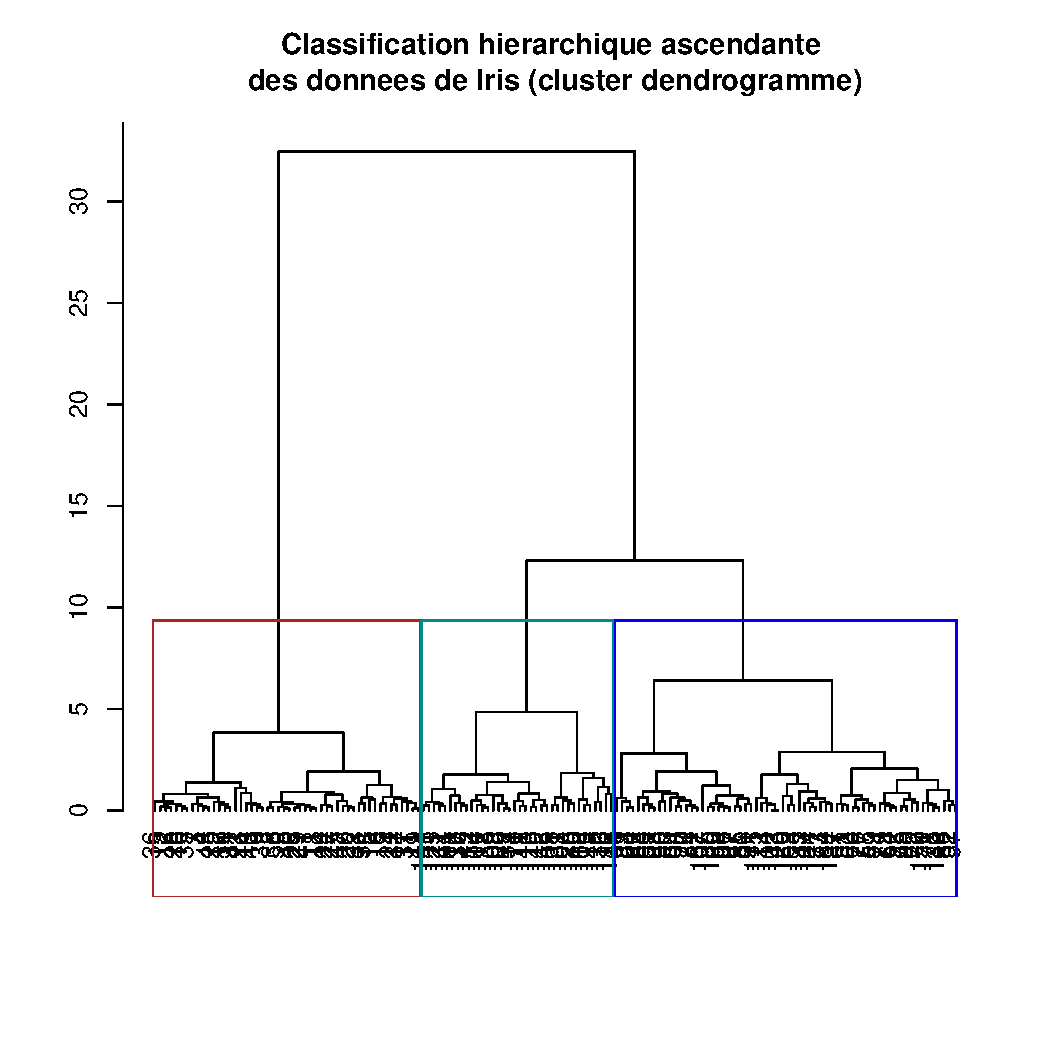
\includegraphics[width=0.35\textwidth]{Iris_cluster_dendrogramme_ascendante.pdf}
    \captionof{figure}{Dendrogramme du CAH avec la méthode de Ward (données Iris)}\label{cha_iris_ward}
\endgroup

\begingroup
   \centering
   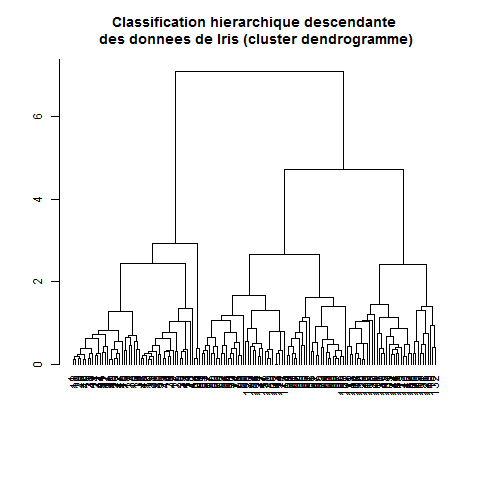
\includegraphics[width=0.35\textwidth]{Iris_cluster_dendrogramme_descendante.png}
    \captionof{figure}{Dendrogramme du CDH avec la méthode de Ward (données Iris)}\label{chd_iris_ward}
\endgroup

Enfin, on réalise une Classification Descendante Hiérarchique (CDH) sur le jeu de données \texttt{Iris}. A titre de rappel, à contrario de la CAH, au départ, tous les individus sont dans une seule et même classe. Puis, on divise cette classe en $2$ classes. Ensuite, on réitère le processus sur chacune des classes jusqu'à ce que chacune d'entre elles contiennent un et un seul individu. Afin d'y parvenir, nous avons utilisé la fonction \texttt{Diana} de la bibliothèque \texttt{cluster} (figure \ref{chd_iris_ward}).

On peut remarquer que le résultat (figure \ref{chd_iris_ward}) est très proche de celui obtenu avec la CAH (figure \ref{cha_iris_ward}). Il n'y a pas de différences "flagrantes" et nous pouvons à nouveau observer une partition de $2$ classes au sein du dendrogramme. Cette partition contient une classe constituée des individus des deux espèces difficilement différentiables (branche de droite de la racine dans la figure \ref{chd_iris_ward}) et d'une classe constituée des individus de la troisième espèce (branche de gauche de la racine dans la figure \ref{chd_iris_ward}).

\section{Méthode des centres mobiles}
\label{sec_methode_centres_mobiles}

\subsection{Données Iris}
\label{subsec_methode_centres_mobiles_iris}
Tout d'abord, nous avons commencé par trouver des partitions en $K \in \{2 ; 3 ; 4\}$ classes via l'algorithme des centres mobiles. Les résultats sont respectivement consultables à gauche dans la figure \ref{fig_iris_2_4_clusters}, à droite dans la figure \ref{fig_iris_2_4_clusters} et à gauche dans la figure \ref{fig_iris_31_32_clusters}.

La partition $P_{11}$ en $K = 2$ classes (à gauche dans la figure \ref{fig_iris_2_4_clusters}) est proche de celle prédite dans la sous-section \ref{subsec_visualisation_donnes_iris} : les individus d'une classe ont pour espèce \texttt{setosa} tandis que les individus de l'autre classe sont majoritairement, soit d'espèce \texttt{versicolor}, soit d'espèce \texttt{virginica}.

On constate que la partition $P_{12}$ en $K = 3$ classes (à gauche dans la figure \ref{fig_iris_31_32_clusters}) obtenue via la méthode des centres mobiles est proche de la partition réelle (figure \ref{fig_iris_selon_espece}).

La partition $P_{13}$ en $K = 4$ classes (à droite dans la figure \ref{fig_iris_2_4_clusters}) s'interprète ainsi : les individus d'une classe ont majoritairement pour espèce \texttt{setosa}, les individus d'une deuxième classe sont majoritairement d'espèce \texttt{versicolor}, les individus d'une troisième classe ont majoritairement pour espèce \texttt{virginica} et la quatrième classe est majoritairement constituée d'individus \texttt{versicolor} et \texttt{virginica}.

Afin d'étudier la stabilité du résultat de la partition, nous avons effectué plusieurs classifications des données en $K = 3$ classes. 

A certaines reprises, nous obtenions la partition $P_{14}$ consultable à droite dans la figure  \ref{fig_iris_31_32_clusters}. Cette partition s'interprète ainsi : une classe est majoritairement constituée d'individus \texttt{versicolor} et \texttt{virginica} tandis que les deux autres se sont majoritairement formés à partir des individus \texttt{setosa} restants. La somme des inerties des classes par rapport à leur centre de la partition $P_{14}$ est proche de $0.95$ tandis que la même somme de la partition $P_{12}$ est proche de $0.53$. Ainsi, comme prévu, la partition $P_{12}$ est meilleure que la partition $P_{14}$ au sens du critère mentionné ci-dessus.

\begingroup
	\centering
   \begin{minipage}[c]{0.23\textwidth}
      \centering 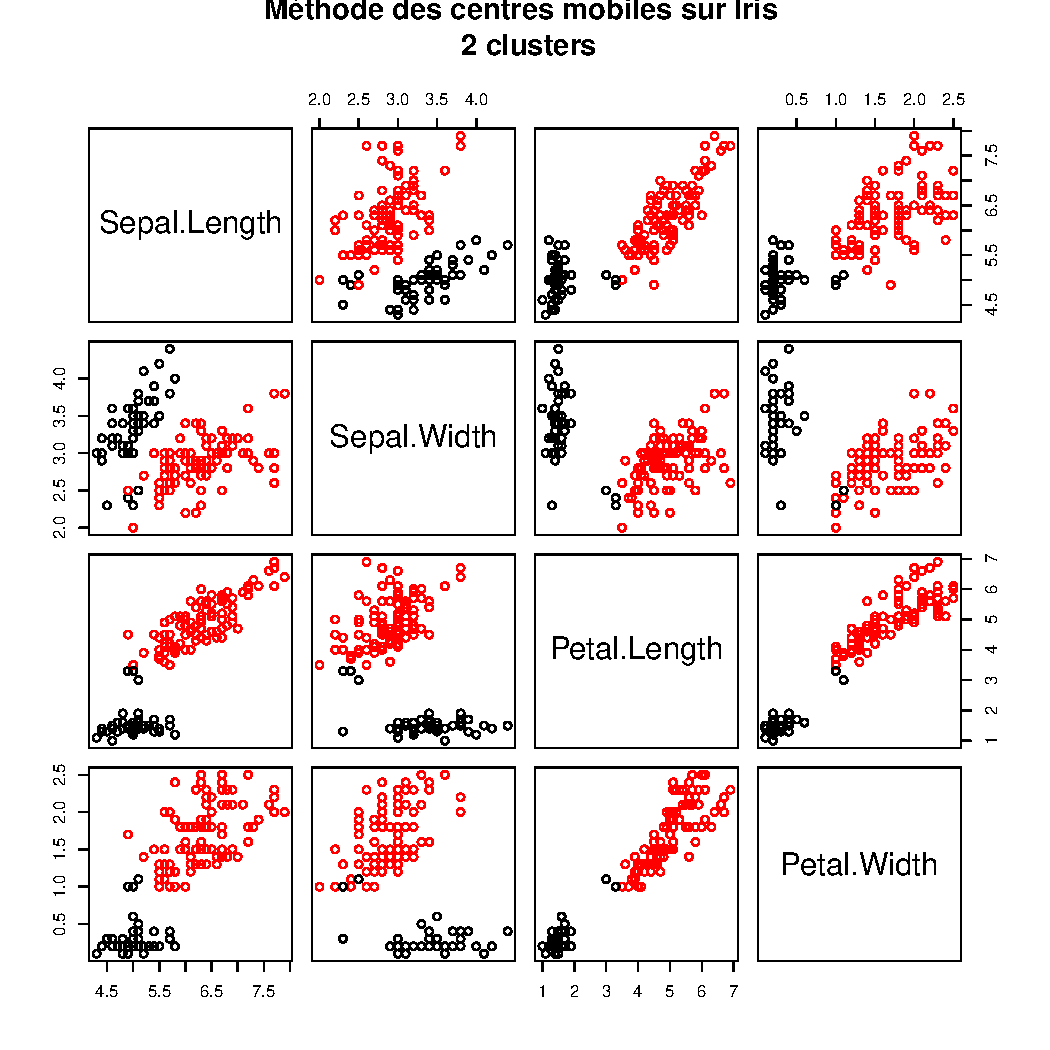
\includegraphics[width=\textwidth]{iris_2_clusters.pdf}
   \end{minipage}\hfill
   \begin{minipage}[c]{0.23\textwidth}   
      \centering 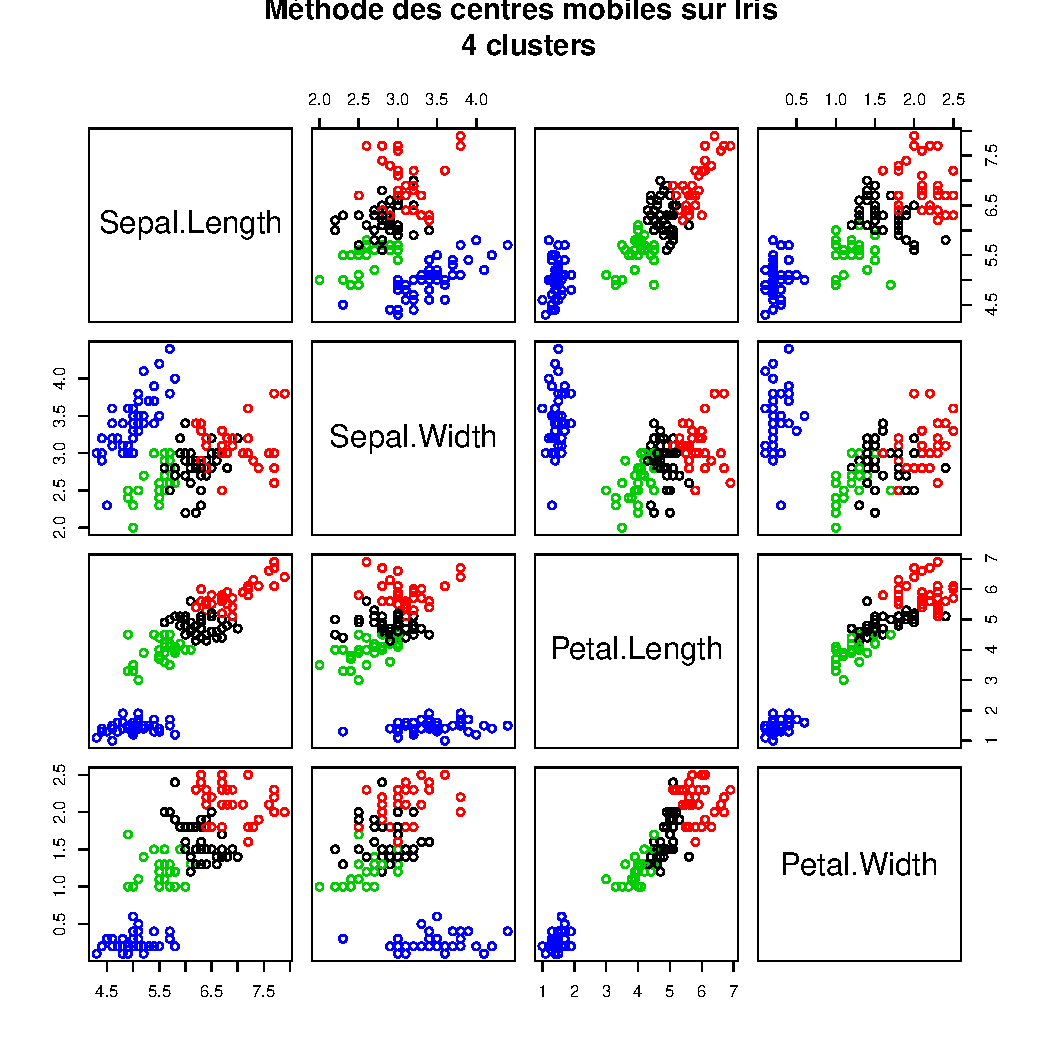
\includegraphics[width=\textwidth]{iris_4_clusters.pdf}
   \end{minipage}
    \captionof{figure}{Partition en 2 classes (à gauche) / en 4 classes (à droite) (Iris)} \label{fig_iris_2_4_clusters}
\endgroup

\begingroup
	\centering
   \begin{minipage}[c]{0.23\textwidth}
      \centering 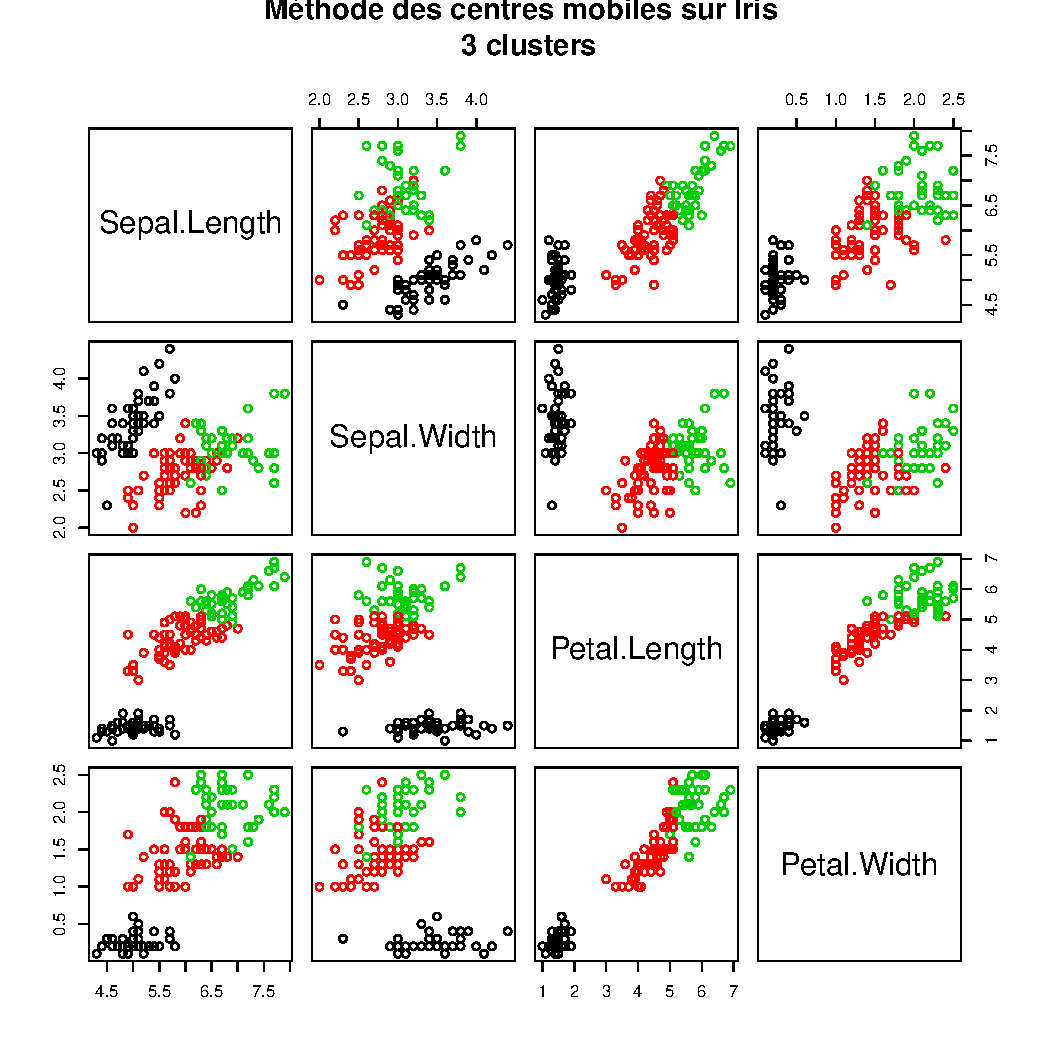
\includegraphics[width=\textwidth]{iris_3_clusters.pdf}
   \end{minipage}\hfill
   \begin{minipage}[c]{0.23\textwidth}   
      \centering 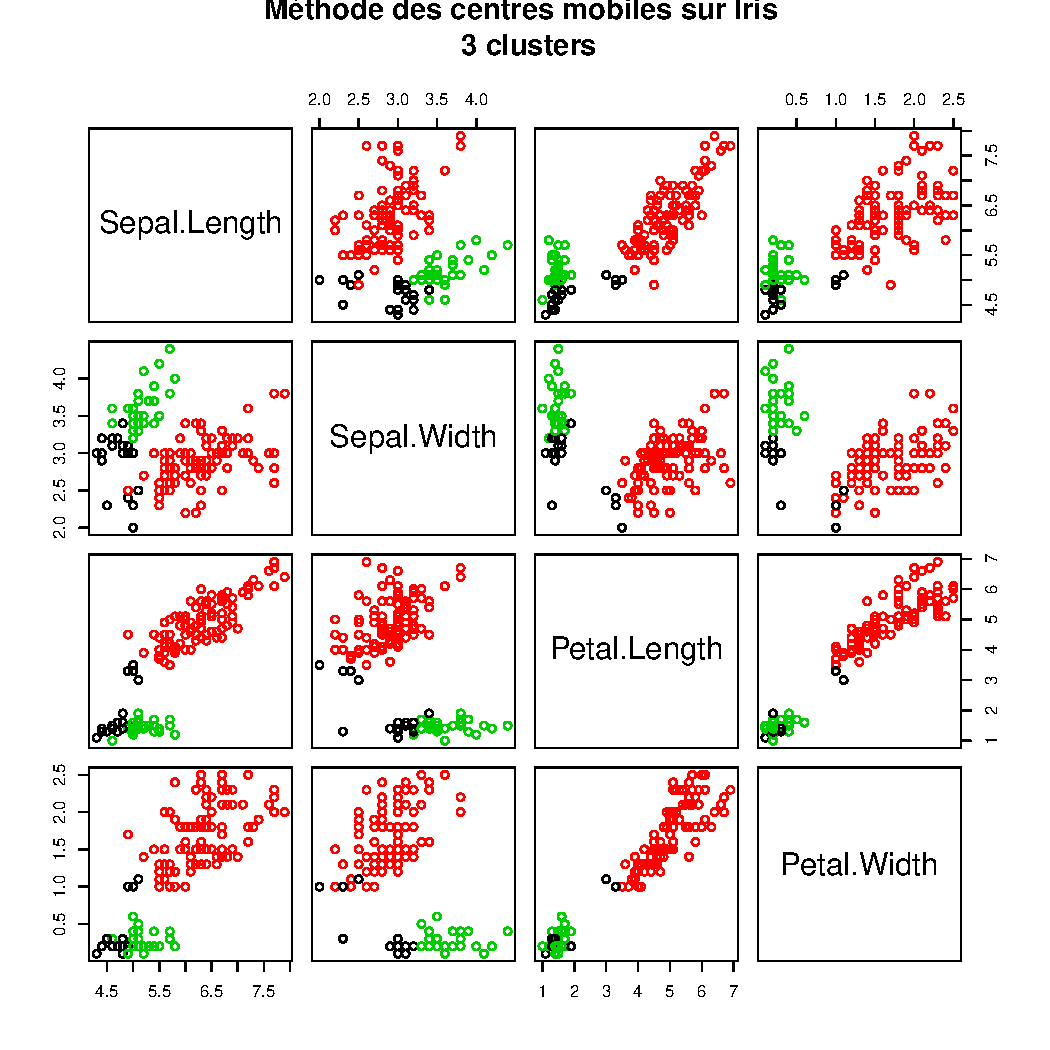
\includegraphics[width=\textwidth]{iris_32_clusters.pdf}
   \end{minipage}
    \captionof{figure}{Partition en 3 classes : première configuration (à gauche) / deuxième configuration (à droite) (Iris)} \label{fig_iris_31_32_clusters}
\endgroup

Cette différence de résultats est facilement explicable : effectivement, l'algorithme des centres mobiles propose une partition visant à minimiser le critère mentionné ci-dessus. Toutefois, suivant les points de départ choisis, les résultats sont différents : l'algorithme converge donc vers un optimum local qui peut-être global. Ainsi, à une reprise, les points de départ choisis ont fait que l'algorithme a convergé vers la partition $P_{12}$. A une autre reprise, d'autres points de départ ont fait que l'algorithme a convergé vers la partition $P_{14}$.

Ensuite, on a cherché à déterminer le nombre de classes $K$ optimal. Pour ce faire, on a effectué $N = 100$ classifications en prenant $K = 2$ classes, puis, à nouveau $N = 100$ classifications en $K = 3$ classes, $K = 4$ classes, $\cdots$, jusqu'à $K = 10$ classes. Ainsi, on a constitué neuf échantillons iid que l'on notera $I_2, \cdots, I_{10}$ contenant chacun $N = 100$ sommes d'inerties intra-classe. Pour chaque valeur de $K, K \in \{2 ; \cdots; 10 \}$, on a calculé la somme minimale d'inertie intra-classe $\hat{I}_{K} = \min_{i = 1, \cdots, 100}(I_{Ki})$. Puis, on a représenté la variation de somme minimale d'inerties $\hat{I}_{K}, K \in \{2 ; \cdots; 10 \}$ en fonction du nombre de classes $K$ dans la figure \ref{fig_mutations_test_2_pourc_iner}. En utilisant la méthode des coudes, nous proposons $2$ comme nombre de classes. 


\begingroup
   \centering
   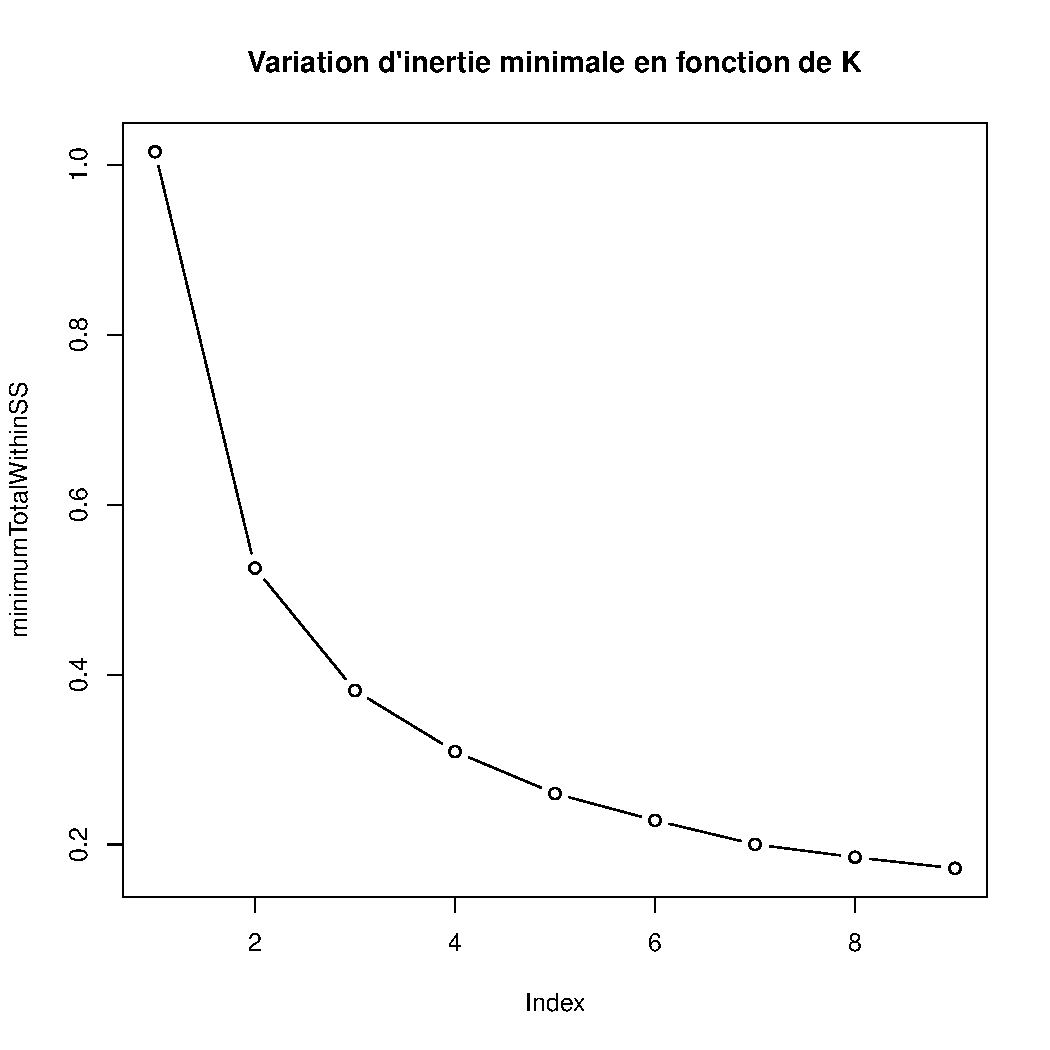
\includegraphics[width=0.35\textwidth]{iris_variation_inertie_min.pdf}
    \captionof{figure}{Variation de la somme minimale d'inerties intra-classe en fonction du nombre de classes (Iris)}\label{fig_mutations_test_2_pourc_iner}
\endgroup

Le nombre de classes $K = 2$ proposé avec la méthode des coudes est celui prédit graphiquement dans la sous-section \ref{subsec_visualisation_donnes_iris}. Par ailleurs, si on calcule la somme des inerties intra-classe de la partition réelle, on constate qu'elle est proche de $0.60$. Évidemment, l'inertie de la partition à deux classes obtenue à l'aide de l'algorithme des centres mobiles est plus élevée, proche de $1.02$. Cependant, on constate que la même inertie pour la partition à trois éléments obtenue avec la même méthode est proche de $0.53$ : elle est inférieure à celle de la partition réelle. En cherchant à minimiser le critère, l'algorithme s'est permis de déplacer certains individus vers des classes différentes de leurs classes d'origine.


\subsection{Données Crabs}
\label{subsec_methode_centres_mobiles_crabs}
Afin d'étudier la stabilité de la partition à $2$ classes, nous avons effectué plusieurs classifications des données en $K = 2$ classes. A certaines reprises, nous obtenions la partition $P_{21}$ consultable à gauche dans la figure \ref{fig_crabs_21_22_clusters}. Cette partition s'interprète ainsi : une classe est majoritairement constituée d'individus \texttt{O}  tandis que l'autre est majoritairement formée à partir des individus \texttt{B} restants. D'autres fois, nous obtenions la partition $P_{22}$ consultable à droite dans la figure \ref{fig_crabs_21_22_clusters}. Cette partition s'interprète ainsi : une classe est majoritairement constituée d'individus \texttt{F} tandis que l'autre est majoritairement formée à partir des individus \texttt{M} restants.

La somme des inerties intra-classe de la partition $P_{21}$ est proche de $1.29 * 10^{-3}$ tandis que la même somme de la partition $P_{22}$ est proche de $1.78 * 10^{-3}$. Ainsi, comme prévu, la partition $P_{21}$ est meilleure que la partition $P_{22}$ au sens du critère mentionné ci-dessus. On notera également que la partition $P_{21}$ en $2$ classes (à gauche dans la figure \ref{fig_crabs_21_22_clusters}) est proche de celle prédite dans la sous-section \ref{subsec_visualisation_donnes_crabs}.

\begingroup
	\centering
   \begin{minipage}[c]{0.23\textwidth}
      \centering 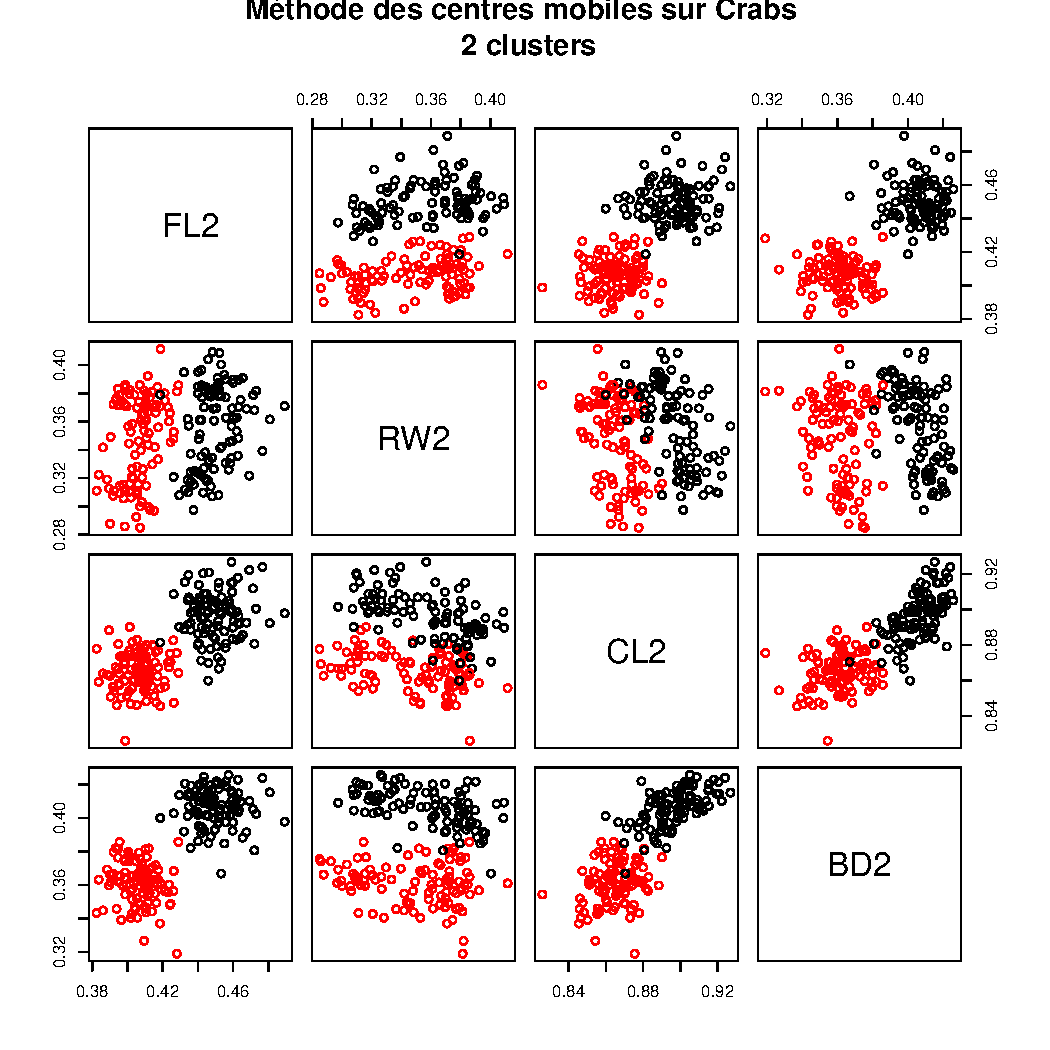
\includegraphics[width=\textwidth]{crabs_21_clusters.pdf}
   \end{minipage}\hfill
   \begin{minipage}[c]{0.23\textwidth}   
      \centering 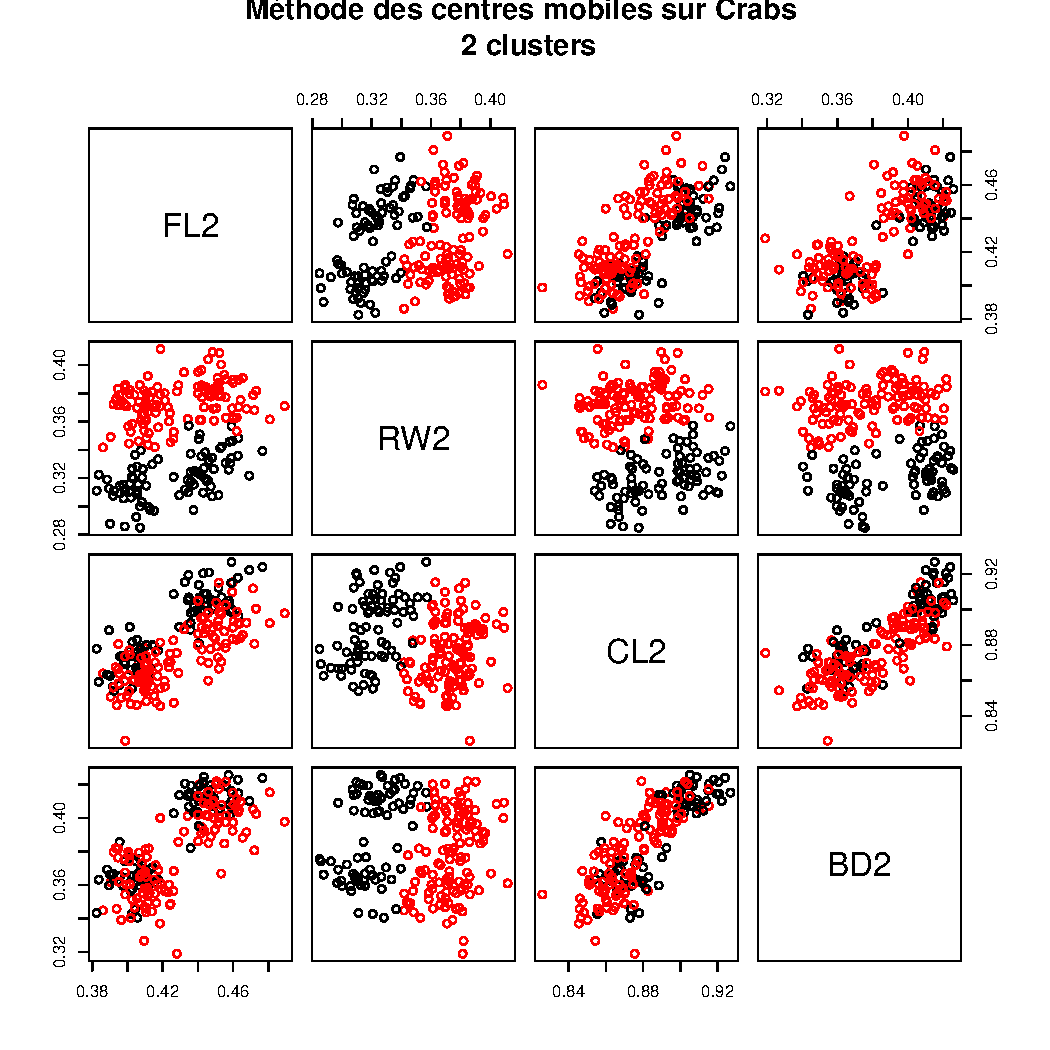
\includegraphics[width=\textwidth]{crabs_22_clusters.pdf}
   \end{minipage}
    \captionof{figure}{Partition en 2 classes : première configuration (à gauche) / deuxième configuration (à droite) (Crabs)} \label{fig_crabs_21_22_clusters}
\endgroup


Ensuite, on a également tenté d'effectuer une classification $P_{23}$ en $K = 4$ classes des données \texttt{Crabs}. Le résultat obtenu est consultable dans la figure \ref{fig_crabs_4_clusters}.

\begingroup
   \centering
   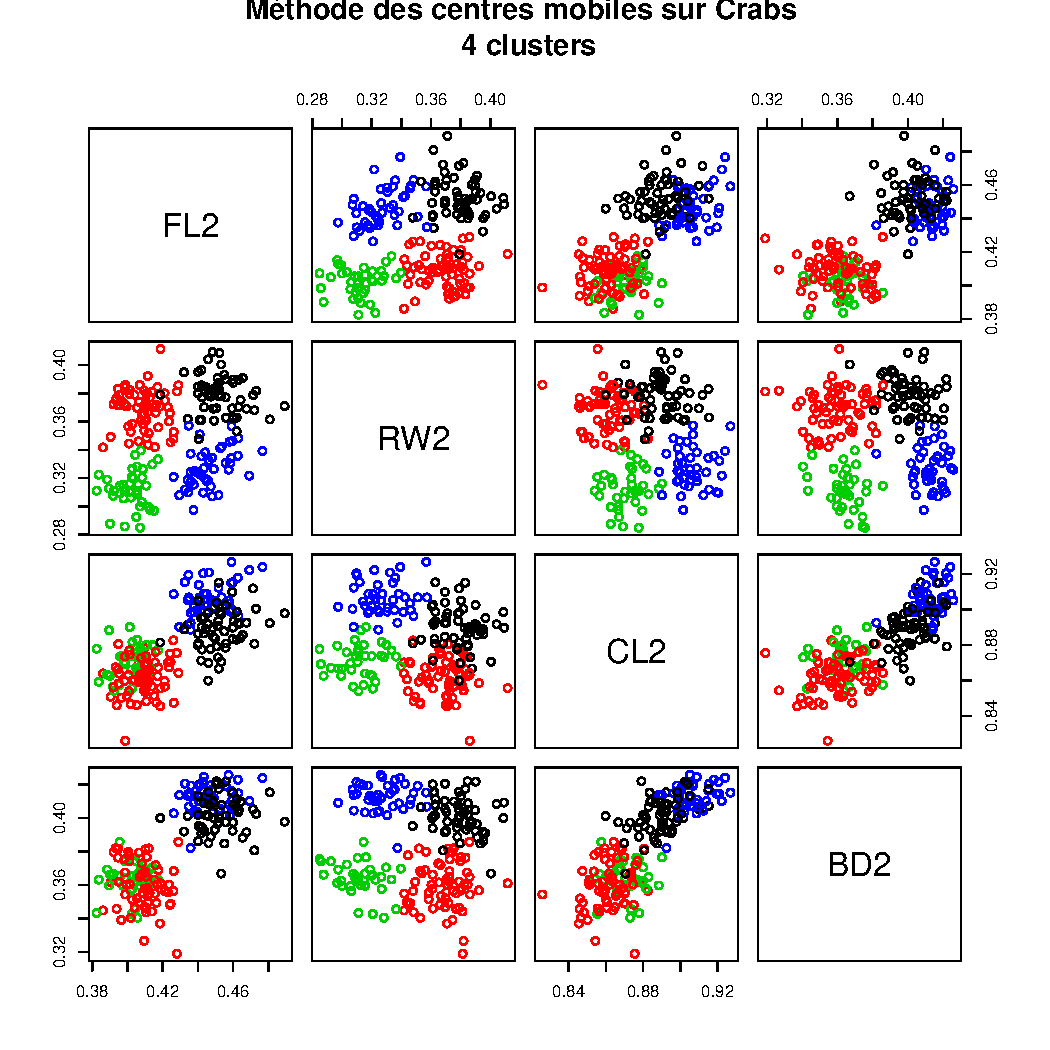
\includegraphics[width=0.35\textwidth]{crabs_4_clusters.pdf}
    \captionof{figure}{Partition en 4 classes (Crabs)}\label{fig_crabs_4_clusters}
\endgroup

On constate que la partition $P_{23}$ en $4$ classes (figure \ref{fig_crabs_4_clusters}) obtenues via la méthode des centres mobiles est proche de la partition réelle (figure \ref{fig_crabs_selon_sexe_et_espece}). Effectivement, la partition s'organise ainsi : chacune des $4$ classes est majoritairement respectivement constituée de \texttt{F/O}, \texttt{M/O}, \texttt{F/B} et de \texttt{F/B}.

Par ailleurs, si on calcule la somme des inerties intra-classe de la partition réelle, on constate qu'elle est proche de $6.24 * 10^{-4}$. Cependant, on constate que la même inertie pour la partition en $4$ classes obtenue avec l'algorithme des centres mobiles est proche de $5.30 * 10^{-4}$ : elle est donc inférieure à celle de la partition réelle. En cherchant à minimiser le critère, l'algorithme s'est à nouveau autoriser à déplacer certains individus vers des classes différentes de leur classe d'origine.

\subsection{Données Mutations}
\label{subsec_methode_centres_mobiles_mutations}
Tout d'abord, nous avons tenté de calculer la représentation des données \texttt{Mutations} dans un espace de dimension $d = 5$.

Ensuite, sur cette représentation, on a effectué $10$ classifications en $K = 3$ classes via l'algorithme des centres mobiles.  Sur ces $10$ classifications, nous avons obtenu $4$ partitions différentes ayant les sommes d'inertie intra-classe suivantes : $245.90$, $181.09$, $248.75$ et $261.86$. Le résultat obtenu pour la partition d'inertie $181.09$ dans le premier plan factoriel de l'\texttt{AFTD} est consultable dans la figure \ref{fig_mutations_dim_5_11}.

\begingroup
   \centering
   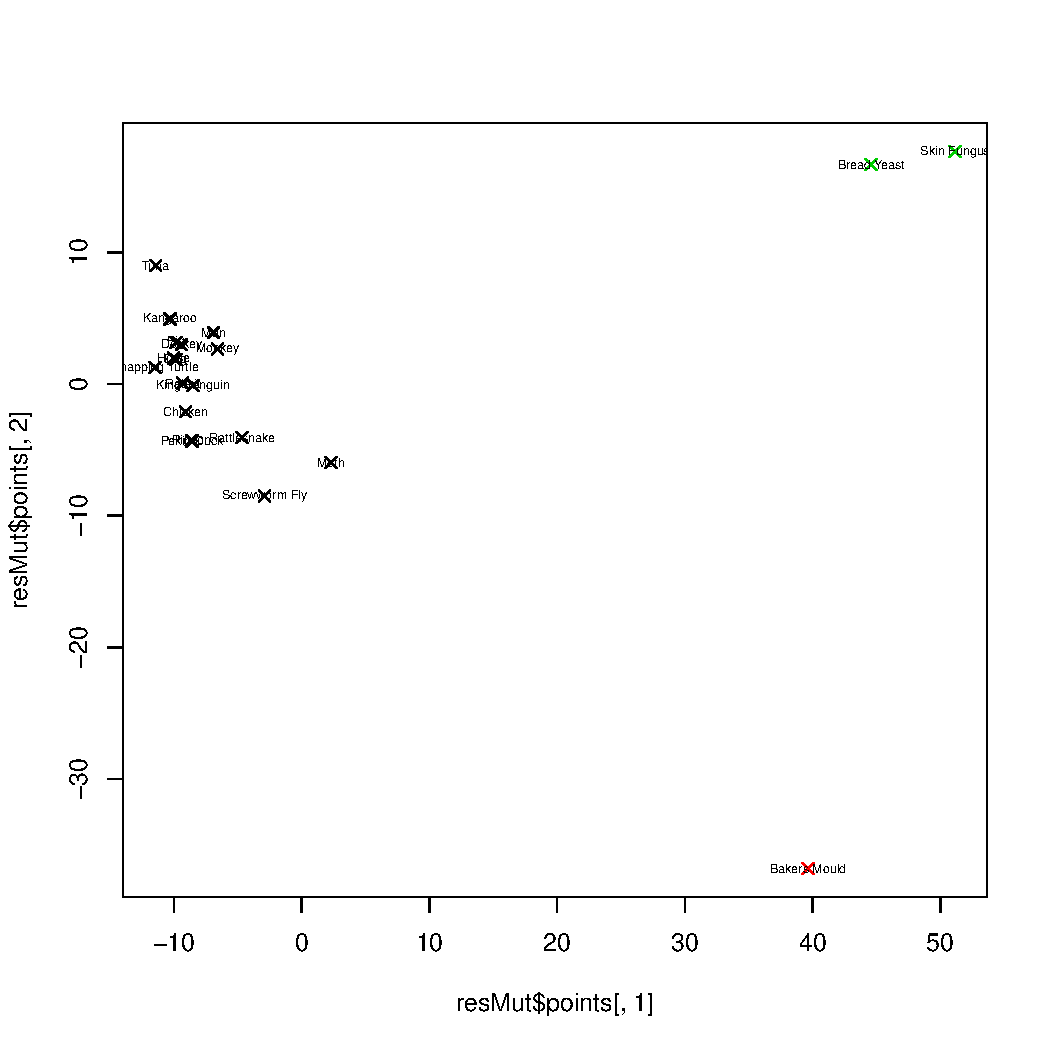
\includegraphics[width=0.35\textwidth]{mutations_dim_5_11.pdf}
    \captionof{figure}{Partition en 3 classes (Mutations)}\label{fig_mutations_dim_5_11}
\endgroup

La partition obtenue (figure \ref{fig_mutations_dim_5_11}) dans le premier plan factoriel de l'\texttt{AFTD} s'avère être particulièrement intuitive. 

Au premier abord, avec ses $4$ partitions différentes sur $10$ classifications, la classification en $K = 3$ classes semble peu stable compte tenu de la "dissimilarité importante" entre deux individus appartenant à deux classes différentes parmi les trois classes obtenues (figure \ref{fig_mutations_dim_5_11}). Toutefois, ce phénomène peut probablement se justifier par le fait que la représentation dans le premier plan factoriel peut masquer ou accentuer certaines dissimilarités entre deux individus (visibles dans d'autres dimensions). Par ailleurs, il est également possible que le fait que la matrice de dissimilarités, avec laquelle on travaille, ne soit pas une matrice de distances, impacte négativement la qualité de la représentation des données obtenues par l'\texttt{AFTD} provoquant ainsi une baisse de la stabilité de l'algorithme. 

\section{Conclusion}
En conclusion, au cours des trois séances de travaux dirigés et de la rédaction du présent rapport, nous avons pu à nouveau prendre conscience de la puissance et des multiples possibilités qui s’offrent à nous en terme de traitement statistique de données avec \texttt{R}. Ainsi, nous avons notamment appris à effectuer une Analyse Factorielle d'un Tableau de Distances (AFTD) en \texttt{R}. Nous avons également eu l'occasion de réaliser des classifications hiérarchiques sur différents jeux de données. Enfin, cela nous a offert la possibilité de tester les performances de la méthode des centres mobiles.
\end{multicols}
\end{document}

% Voir au final où rajouter la partie clustplot pas utiliser (au cas où) + relire intégralité partie 3